\documentclass[compress]{beamer}
\usepackage{hyperref}
\hypersetup{
    pdftitle = {A bird’s-eye view on the habitability of exoplanets via statistical learning techniques}, % <-- Missing in PDF
    pdfauthor = {Marzio De Corato},
    pdfsubject = {Marzio De Corato project the exam: Machine learning, statistical
learning, deep learning and artificial intelligence - Unsupervised Learning}
}

\usepackage[utf8]{inputenc}
\usepackage{graphicx}
\author{Marzio De Corato}
\usepackage{varwidth}
\usepackage{beamerthemesplit} 

\usepackage[english]{babel}
\usepackage[backend=bibtex]{biblatex}
\addbibresource{bibliography.bib}

\useoutertheme{miniframes}


\usetheme[progressbar=frametitle]{Madrid}
\usefonttheme{professionalfonts}
\setbeamertemplate{itemize items}[triangle]
\setbeamertemplate{enumerate items}[default]
\usecolortheme{beaver}


%Information to be included in the title page:


\usebackgroundtemplate{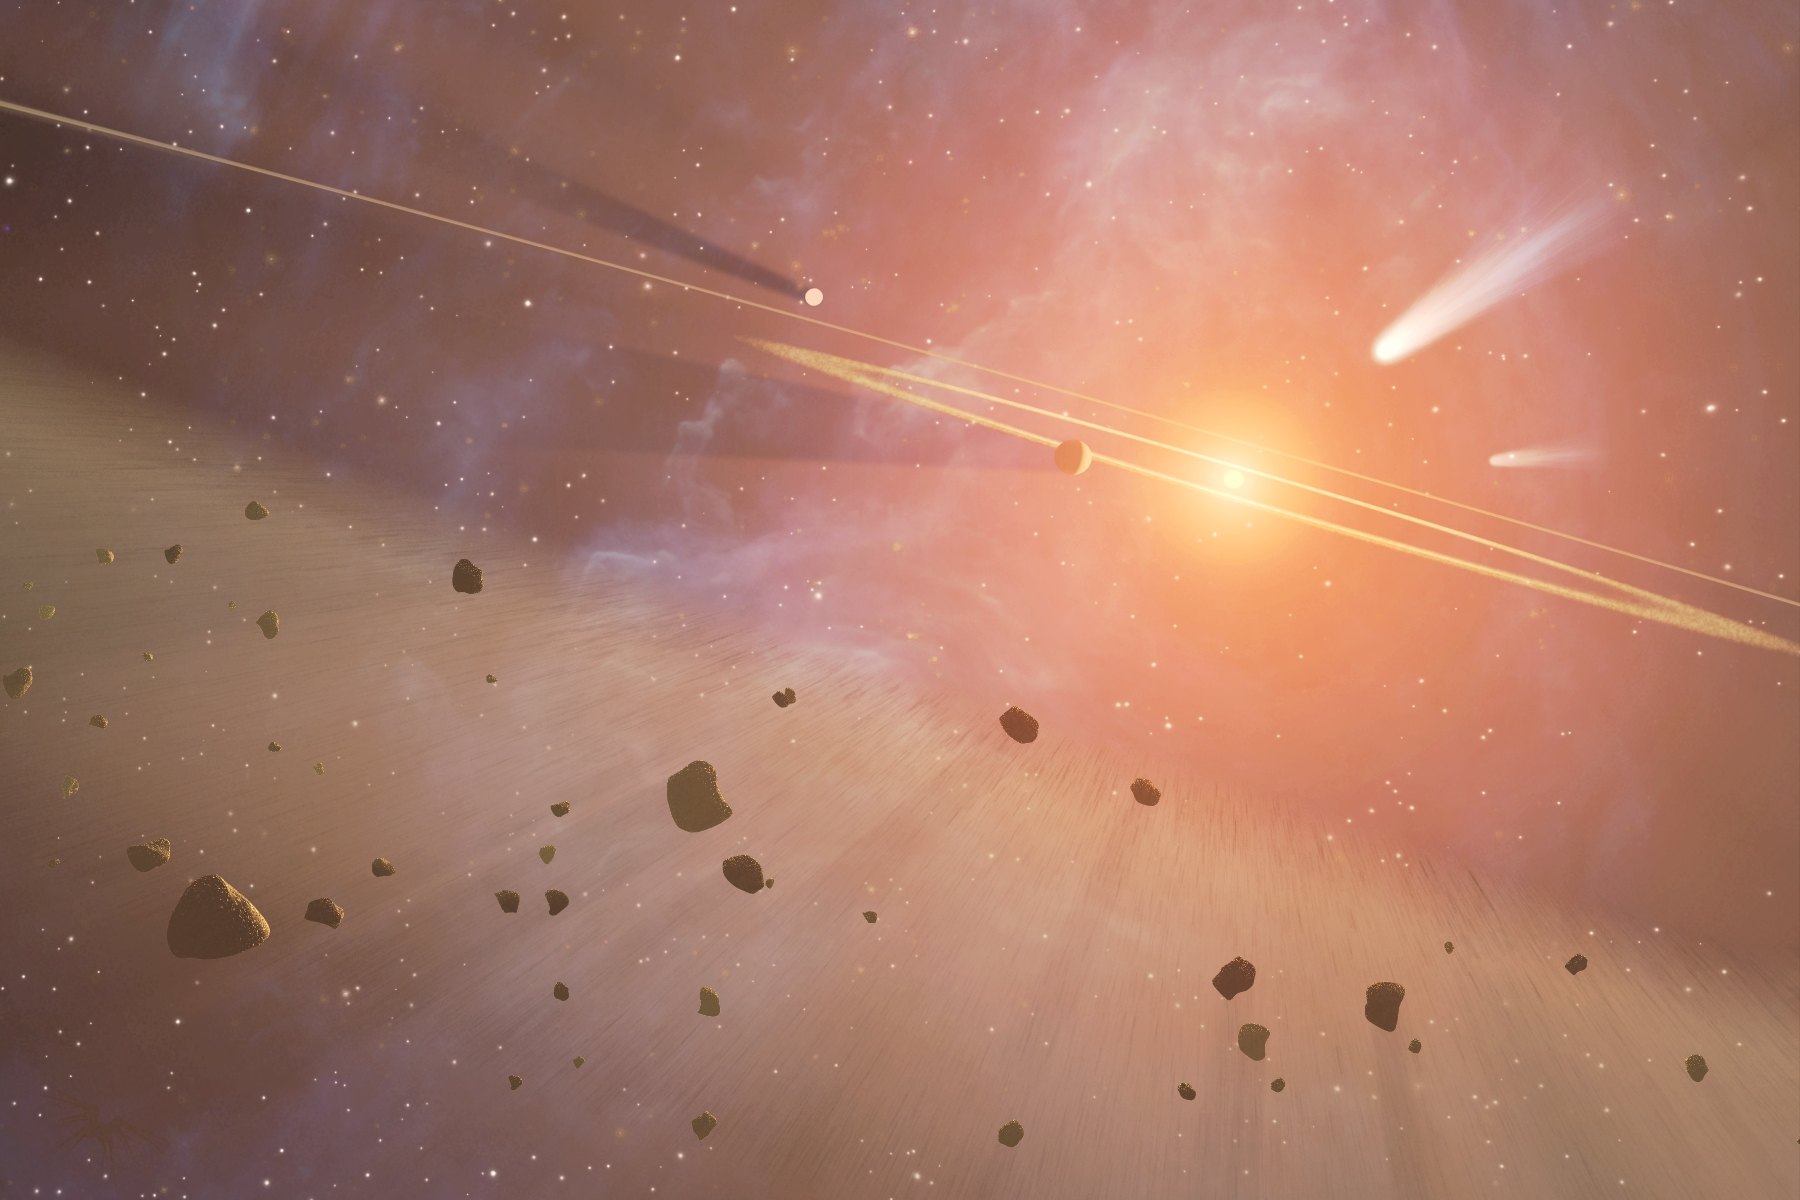
\includegraphics[width=\paperwidth]{Pic/Intro.jpg}}
\title[Exoplanets survey via SL techniques]{A bird’s-eye view on the habitability of exoplanets via statistical learning techniques}

\author{}
\date{}

\subtitle{Project for the exam: Machine learning, statistical
learning, deep learning and artificial intelligence - Unsupervised Learning}

\setbeamertemplate{enumerate items}[default]
\usecolortheme{beaver}

\begin{document}


\frame{\vspace{+4.5cm}\titlepage}

\usebackgroundtemplate{ } 

\author{Marzio De Corato}

\section{Intro}

\begin{frame}
\frametitle{Overview}
\begin{itemize}
\item\textbf{Final goal}: Survey the performances of different statistical learning algorithms for the prediction of exoplanets habitability
\item\textbf{Dataset}: Planetary Habitability Laboratory @ UPR Arecibo \cite{planet_dataset}
\item\textbf{Algorithms}: Decision Tree, Random Forest, Support Vector Classifier, Logistic Regression, Linear and Quadratic Classifier
\end{itemize}
\end{frame}

\section{Theoretical background}
\subsection{Habitability}
\begin{frame}
\frametitle{Theoretical background - Exoplanets habitability }
\begin{columns}
\column{0.5\textwidth}
\begin{itemize}
\item\textbf{Habitability}: Rocky planets where water is present in liquid phase 
\item\textbf{Liquid phase}: At first order, if water is present, the liquid phase is controlled by the surface temperature 
\item\textbf{Atmosphere}: The atmosphere (CO$_{2}$) influences the surface temperature trough the greenhouse effect
\item\textbf{H$_{2}$ and CH$_{4}$}: Other gases such as H$_{2}$ and CH$_{4}$ can produce the greenhouse effect, thus the habitable zone can be extended 
\end{itemize}
\column{0.4\textwidth}
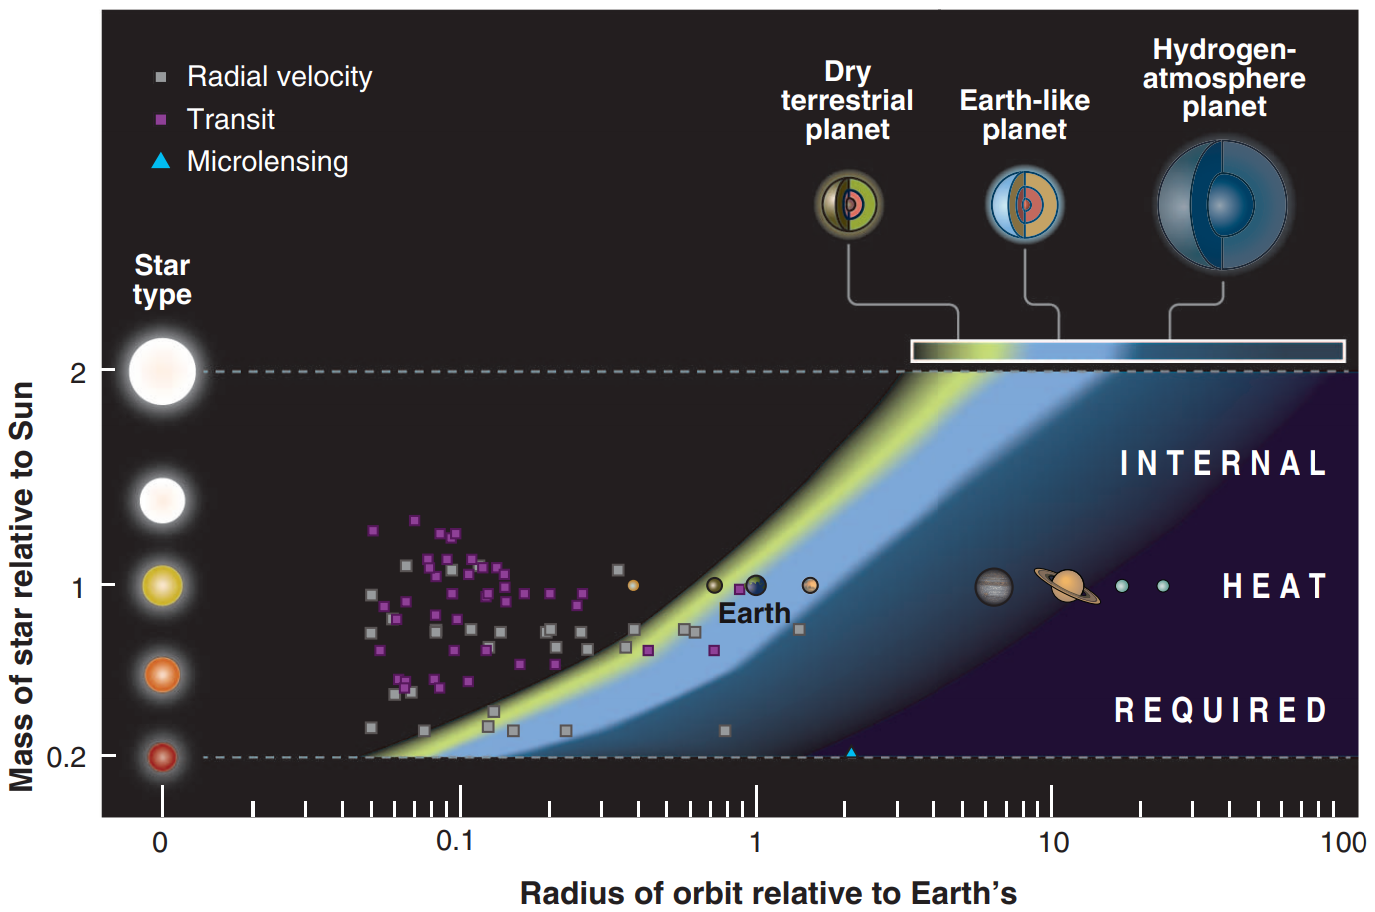
\includegraphics[width=\linewidth,]{Pic/Planets_habitability_Seager.png}\\
\begin{center}
Image taken from \cite{seager2013exoplanet}
\end{center}

\end{columns}
\end{frame}


\subsection{Stars Feature}

\begin{frame}
\frametitle{Theoretical background - Star features }
\begin{columns}
\column{0.4\textwidth}
\begin{itemize}
\item \textbf{Main features}: For this work the main features of star are the stellar luminosity (S\_L), its temperature (S\_T) and spectral type (S\_S\_T)
\item\textbf{H-R diagram}: with these features the Hertzsprung-Russell diagram classify the stars (the temperature and spectral type of a star are two faces of the same medal)
\end{itemize}
\column{0.45\textwidth}
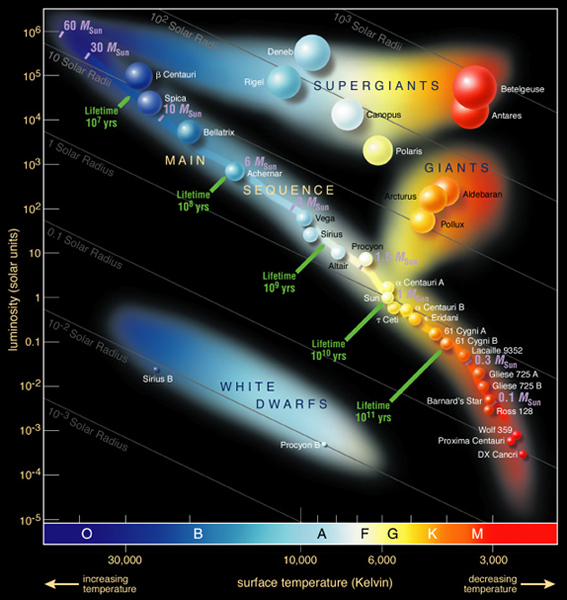
\includegraphics[width=\linewidth,]{Pic/S_T_T_explanation.png}
\begin{center}
Image taken from \cite{HR_diagram}
\end{center}
\end{columns}
\end{frame}

\subsection{Planet Features}

\begin{frame}
\frametitle{Theoretical background - Planet features }
\begin{center}
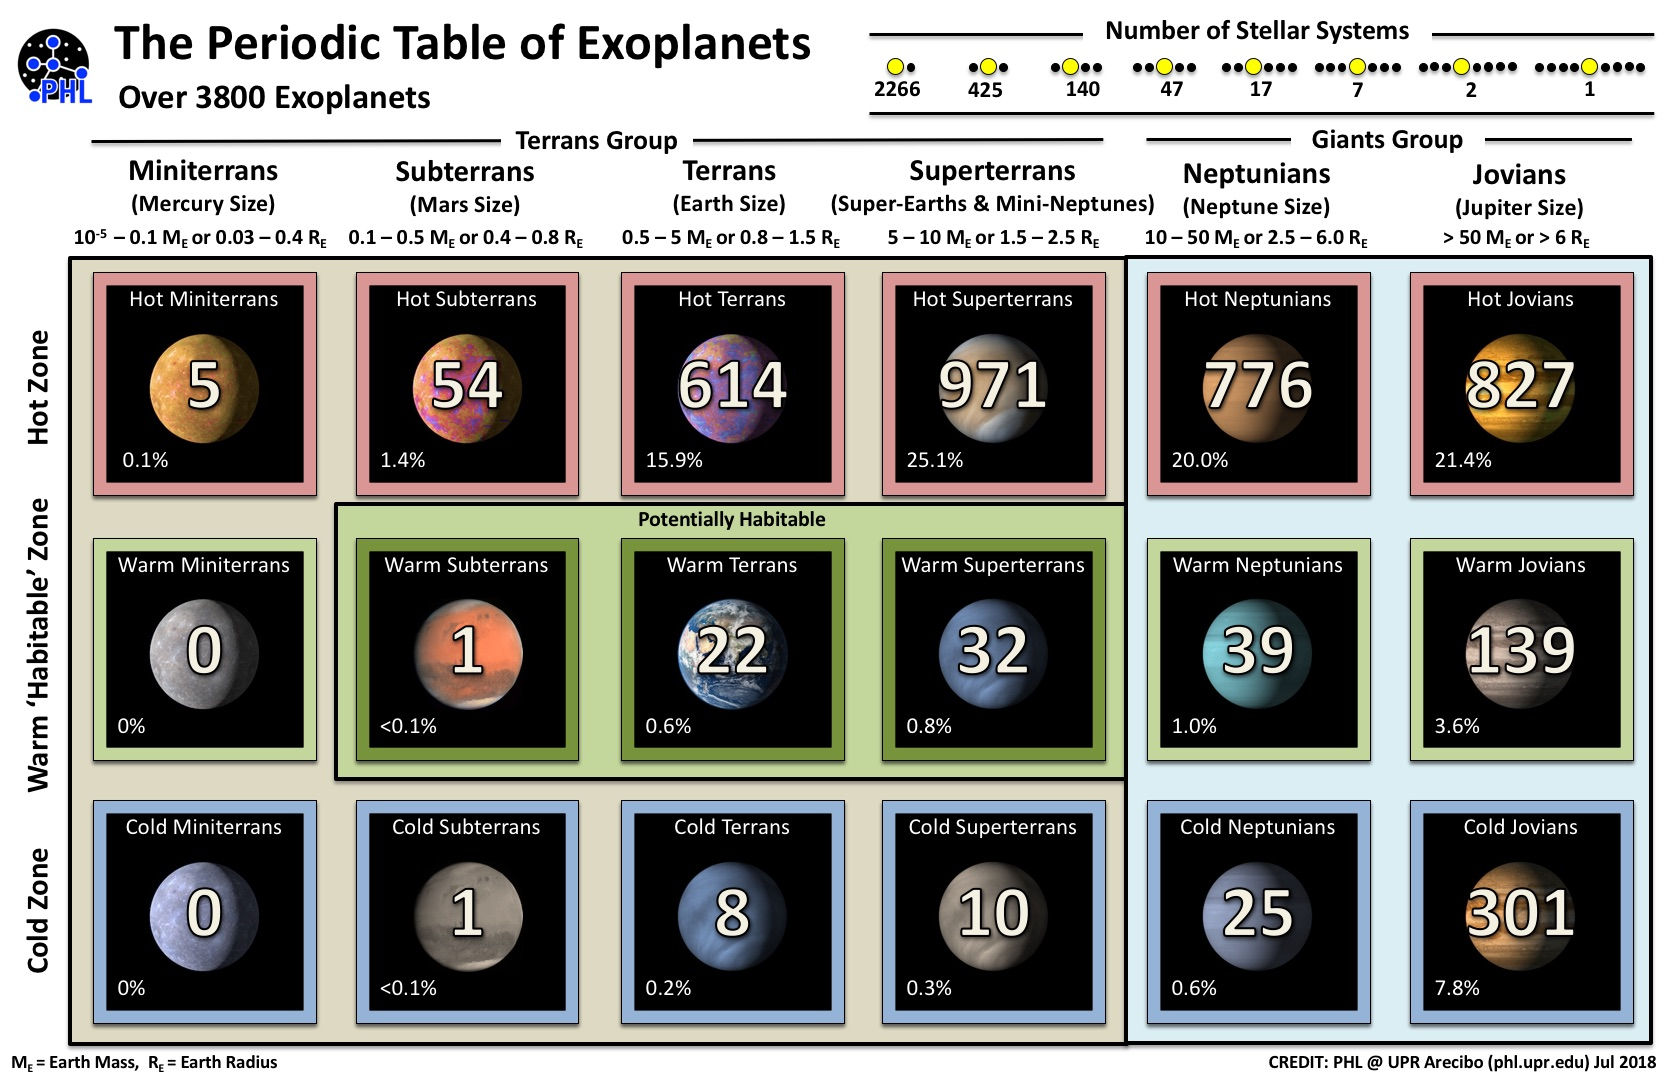
\includegraphics[width=.9\linewidth,]{Pic/PT_Confirmed.jpg}
\end{center}
\begin{center}
Image taken from \cite{exoplanets-catalog}
\end{center}
\end{frame}


\begin{frame}
\frametitle{Theoretical background - Planet features }
\begin{itemize}
\item\textbf{Distance}: in this work the mean planet distance from the host star (P\_D), the periastron (P\_PN) and the apastron (P\_A) as well the termal effective distance (P\_D\_E) from the host star  were considered. These quantities constrain the planet orbital period (P\_P) via the 3$^{th}$ Kepler law (a corollary of Newton's law of universal gravitation)
\item\textbf{Mass and Radius}: the (estimated) planet mass (P\_M) and its radius (P\_R) were considered (these are also useful to distinguish the super-earth planets)
\end{itemize}
\end{frame}
 
\begin{frame}
\frametitle{Theoretical background - Planet features }
\begin{itemize}
\item\textbf{Temperature}: the planet mean stellar flux $P_F$ (defined as $F=S_{L}/4\pi D$, where S$_{L}$ is the host star luminosity and D its distance) and the planet equilibrium temperature (P\_T\_E) were considered. The latter is defined as $T_{eq}=T_{star}\sqrt{R/2a}\left(1-A\right)^{0.25}$) where R is the star radius (S\_R), a the planet mean distance (P\_D), A the albedo (here it was set equal to 0.3)
\item\textbf{Habitability}: The planet habitability was classified with a boolean variable using the values reported in the dataset \cite{planet_dataset}
\end{itemize}
\end{frame}


\section{Data inspection}
\subsection{Densities}
\begin{frame}
\frametitle{Data inspection - densities}
\begin{columns}[t]
        \column{.25\textwidth}
        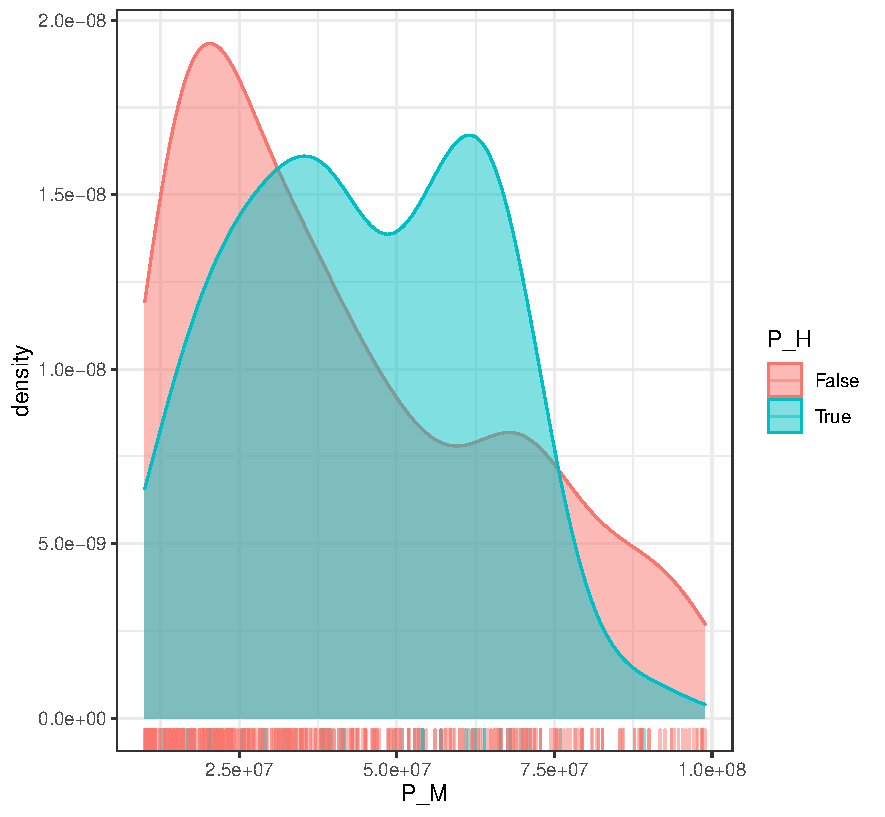
\includegraphics[width=\linewidth]{Pic/Density/P_M.pdf}
        \begin{center}
        Planet mass\\
        \end{center}
        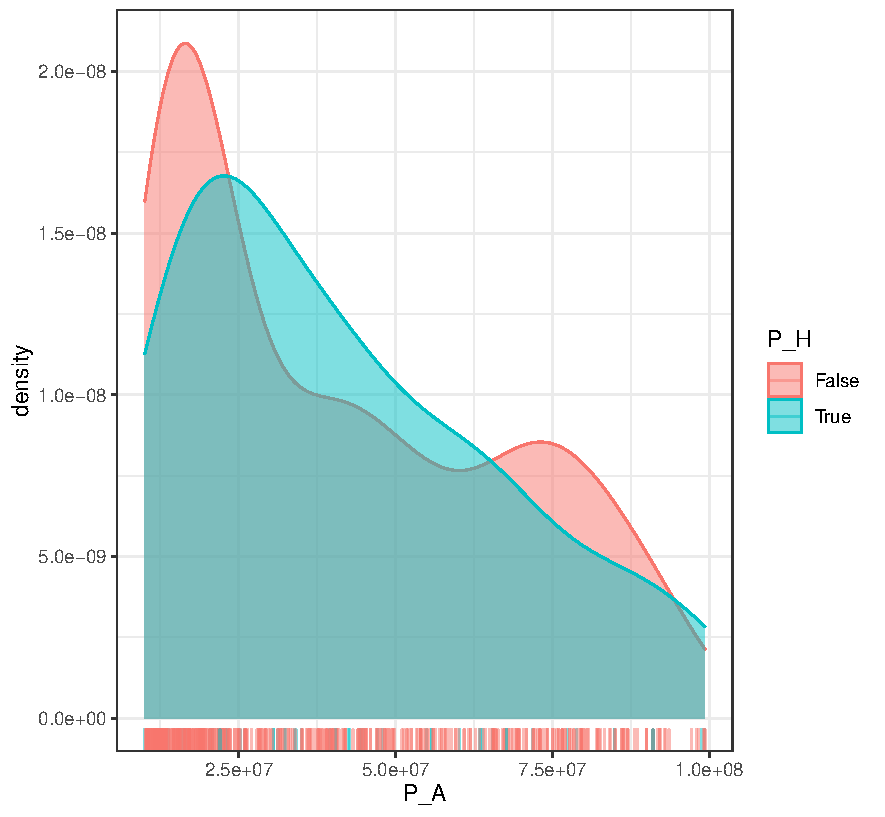
\includegraphics[width=\linewidth]{Pic/Density/P_A.pdf}
        \begin{center}
        Planet apastron\\
        \end{center}
        \column{.25\textwidth}
        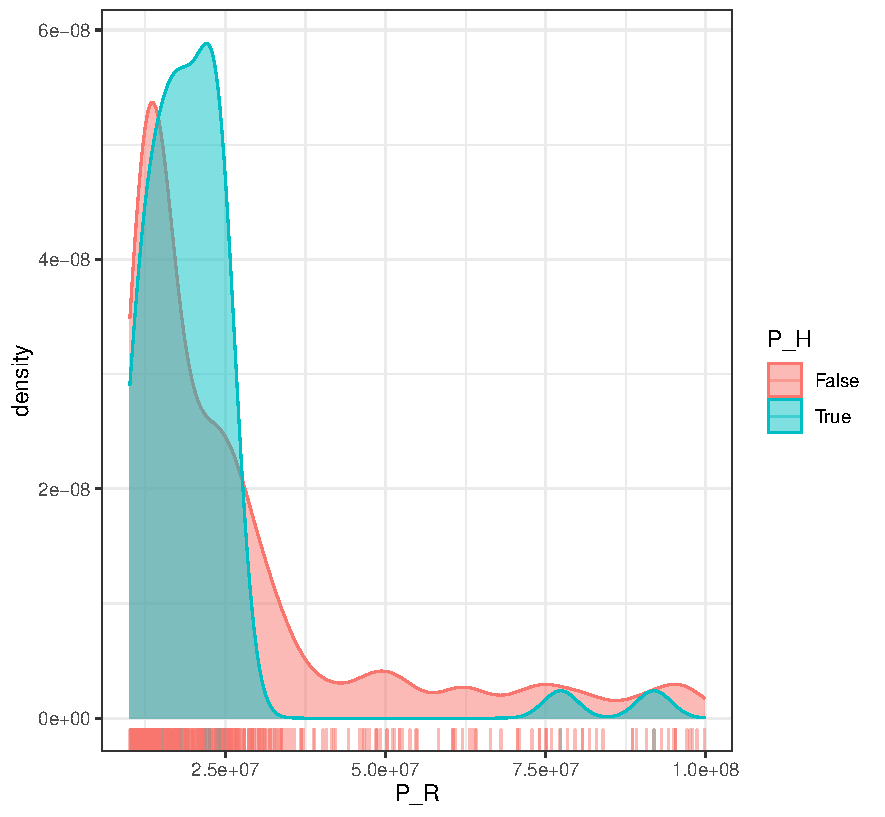
\includegraphics[width=\linewidth]{Pic/Density/P_R.pdf}
        \begin{center}
        Planet radius\\
        \end{center}
        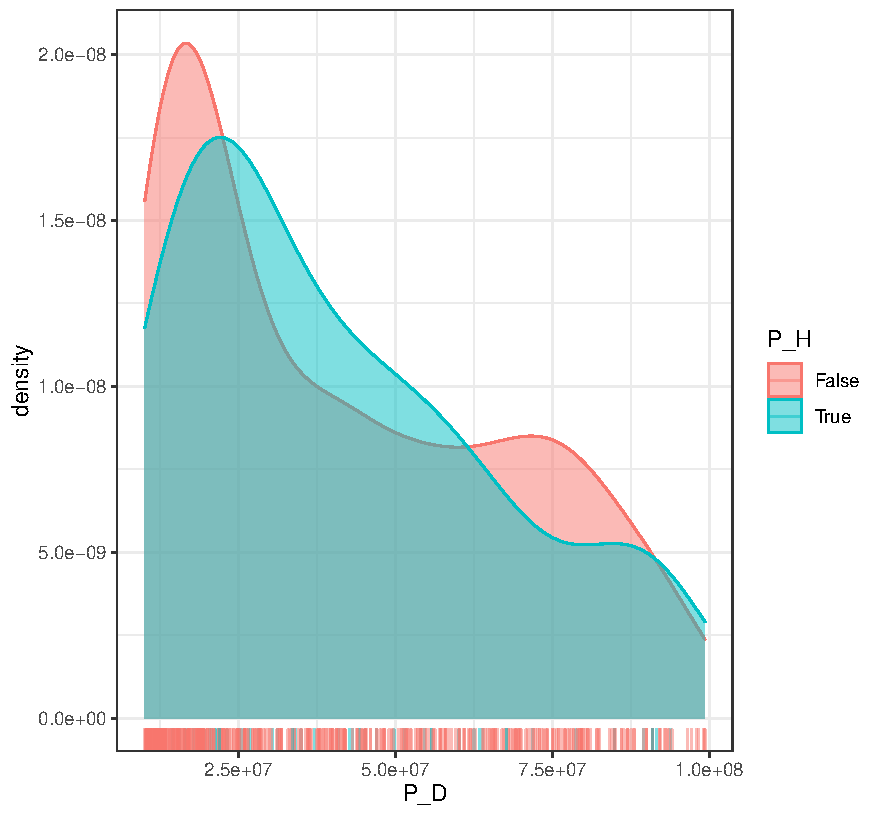
\includegraphics[width=\linewidth]{Pic/Density/P_D.pdf}
        \begin{center}
        Planet distance\\
        \end{center}
        \column{.25\textwidth}
        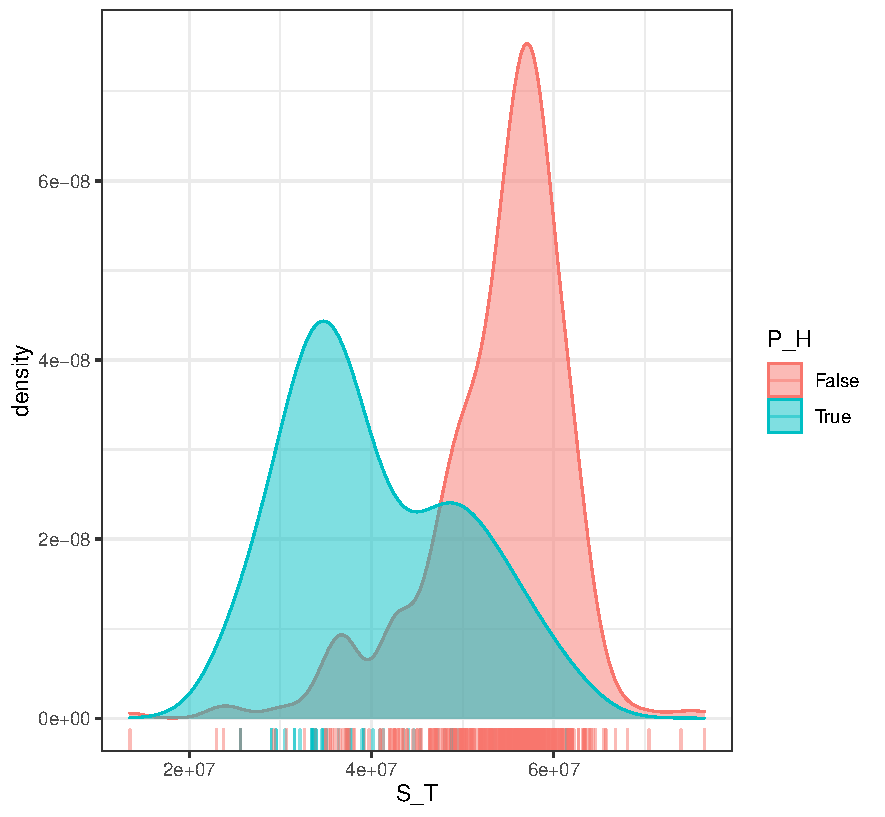
\includegraphics[width=\linewidth]{Pic/Density/S_T.pdf}
        \begin{center}
        Stellar T \\
        \end{center}
        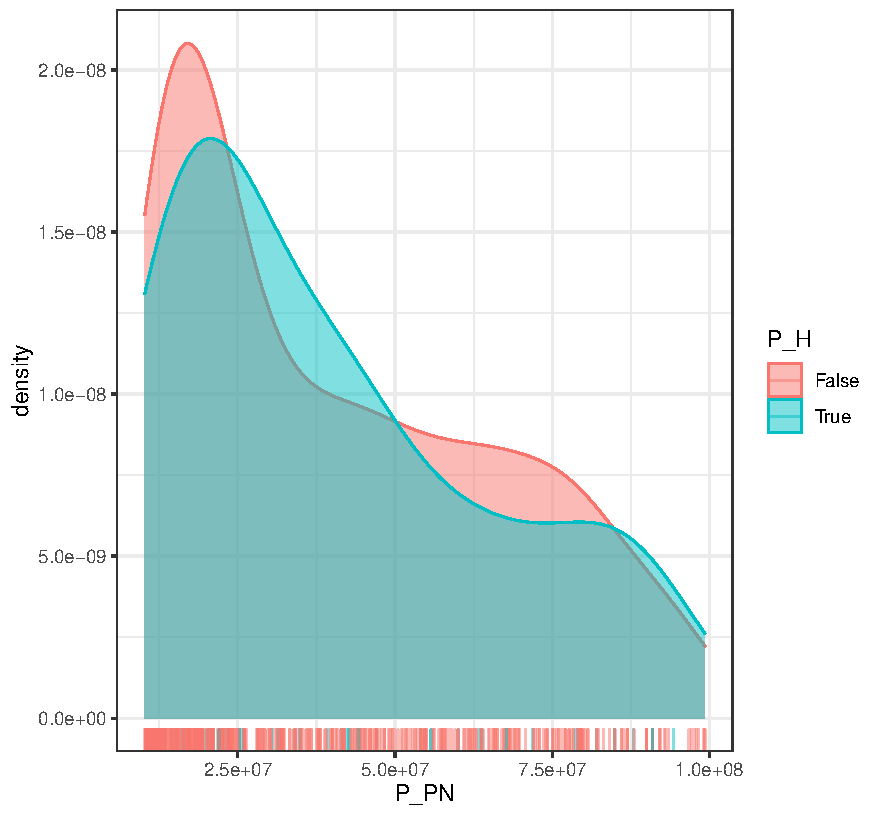
\includegraphics[width=\linewidth]{Pic/Density/P_PN.pdf}
        \begin{center}
        Planet periastron\\
        \end{center}
        \column{.25\textwidth}
        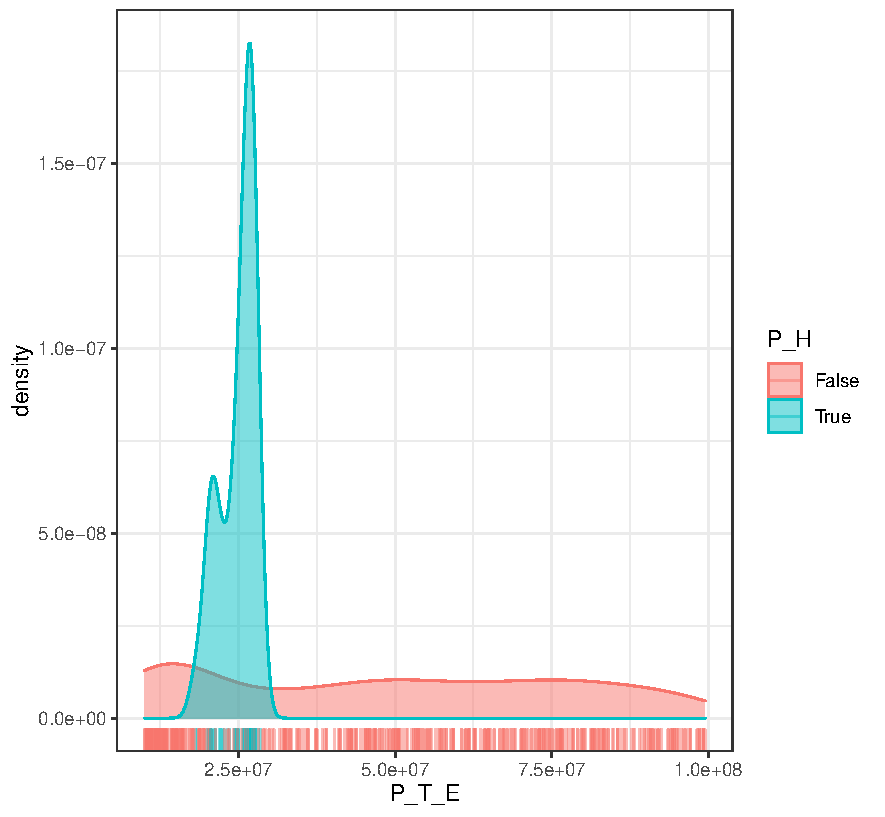
\includegraphics[width=\linewidth]{Pic/Density/P_T_E.pdf}
        \begin{center}
        P T E\\
        \end{center}
        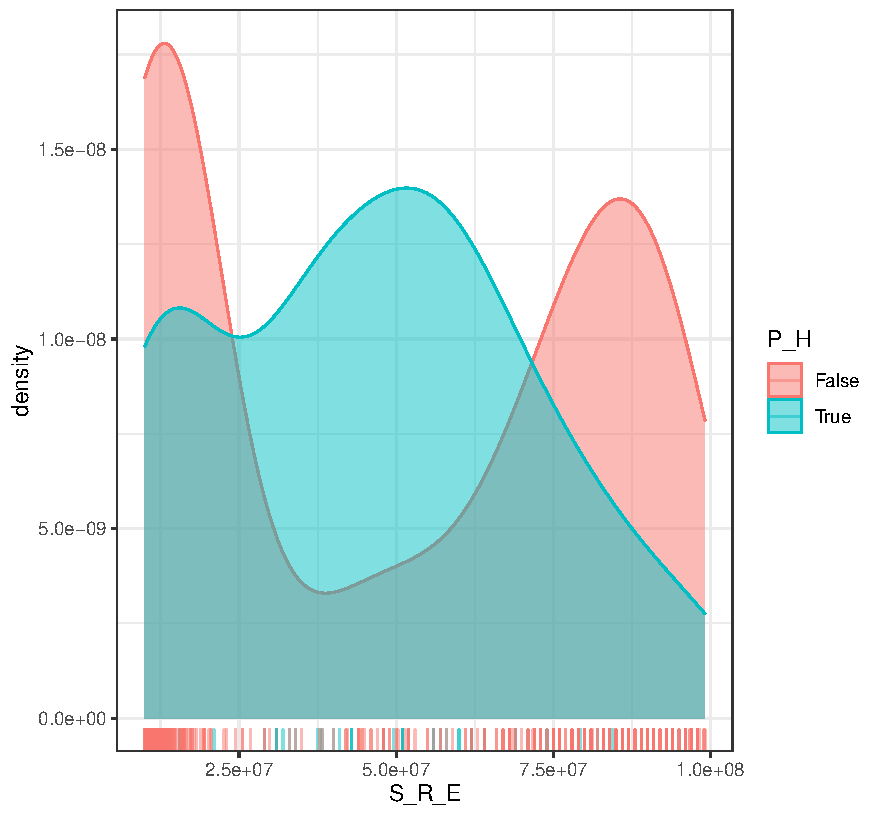
\includegraphics[width=\linewidth]{Pic/Density/S_R_E.pdf}
        \begin{center}
        Star radius\\
        \end{center}
    \end{columns}
\end{frame}

\subsection{FAMD}
\begin{frame}
\frametitle{Data inspection - FAMD}
\begin{columns}
\column{0.5\textwidth}
\begin{center}
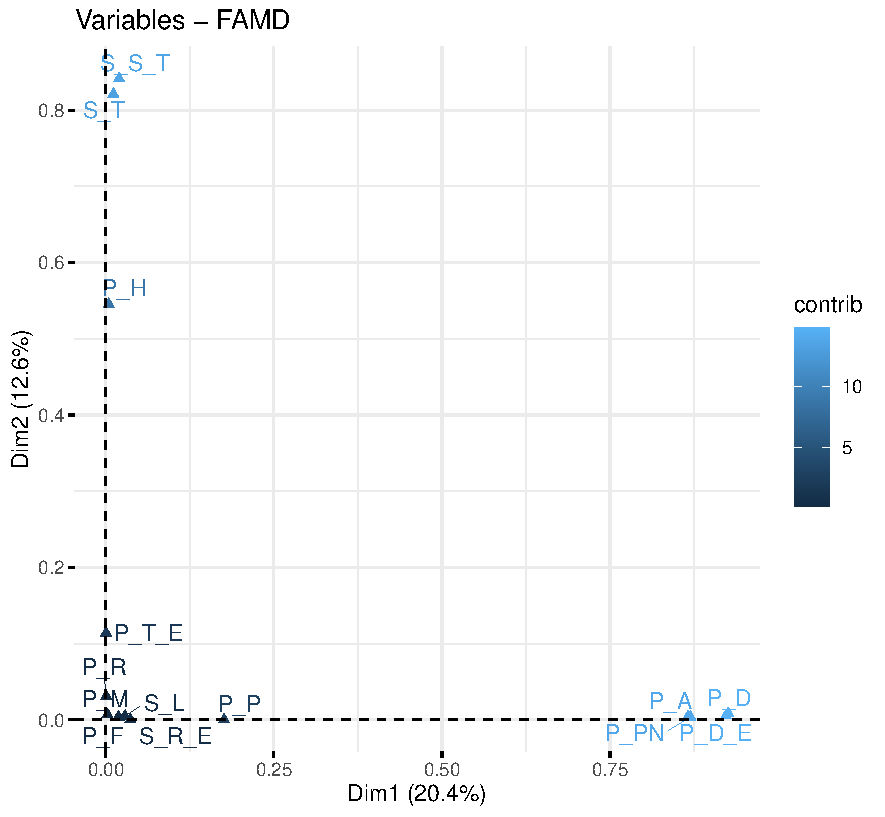
\includegraphics[width=\linewidth]{Pic/FAMD_squared_loadings.pdf}
\end{center}
\column{0.5\textwidth}
\begin{center}
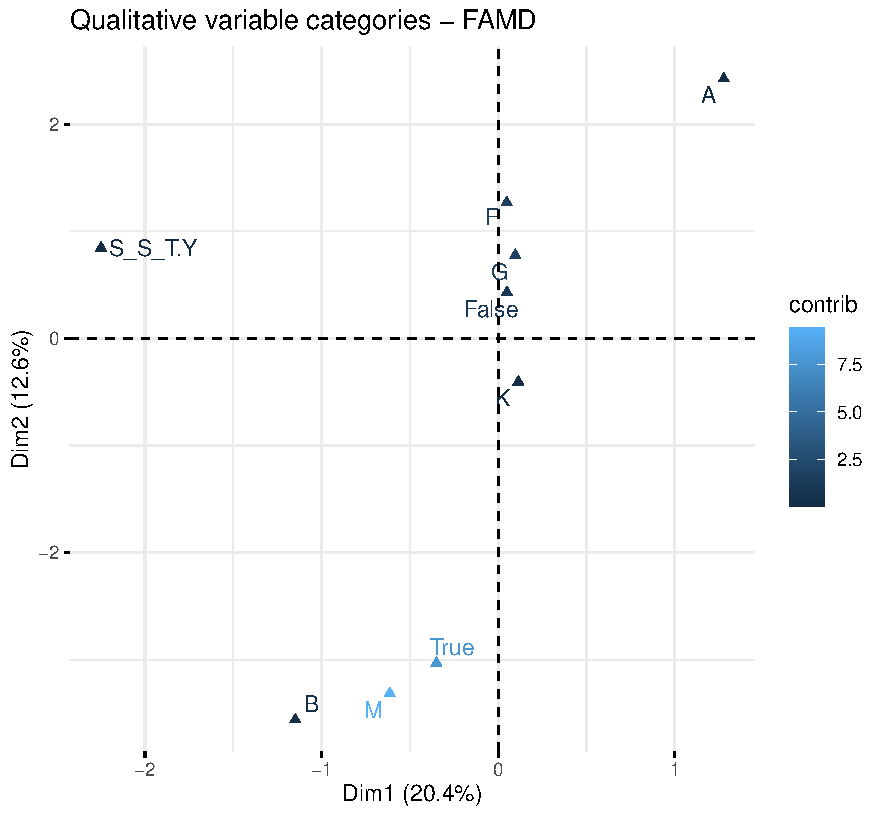
\includegraphics[width=0.7\linewidth]{Pic/FAMD_Qualitative_VAR.pdf}
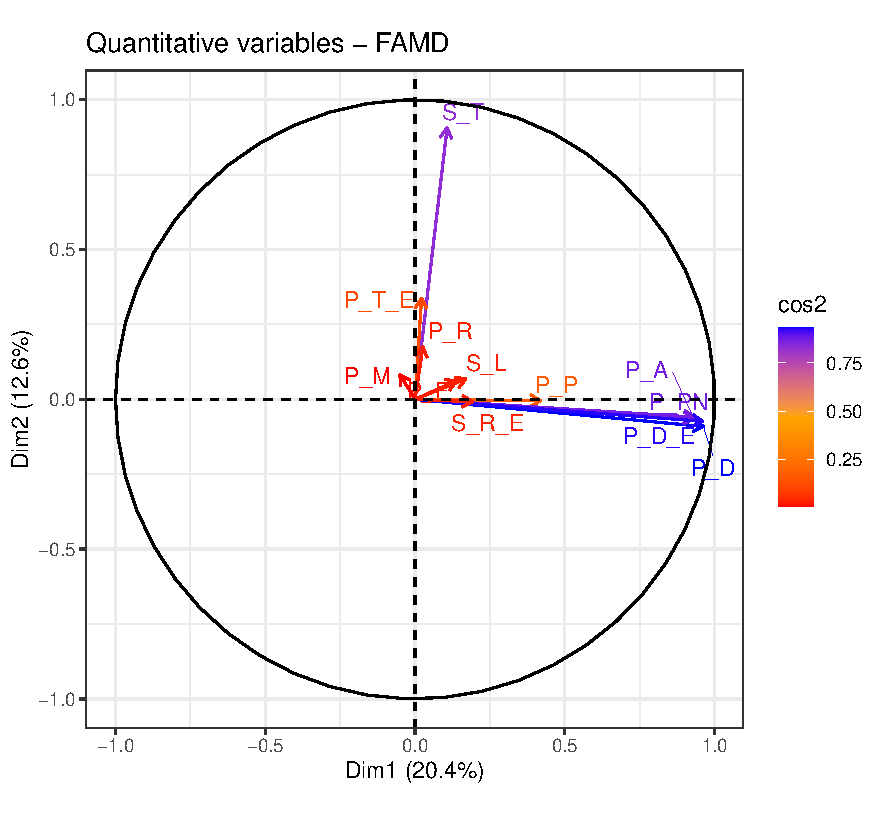
\includegraphics[width=0.7\linewidth]{Pic/FAMD_quantitative_variables.pdf}
\end{center}
\end{columns}
\end{frame}

\section{Results}
\subsection{Results - Decision Tree}
\begin{frame}
\frametitle{Results - Decision Tree}
\begin{columns}
\column{0.5\textwidth}
\begin{center}
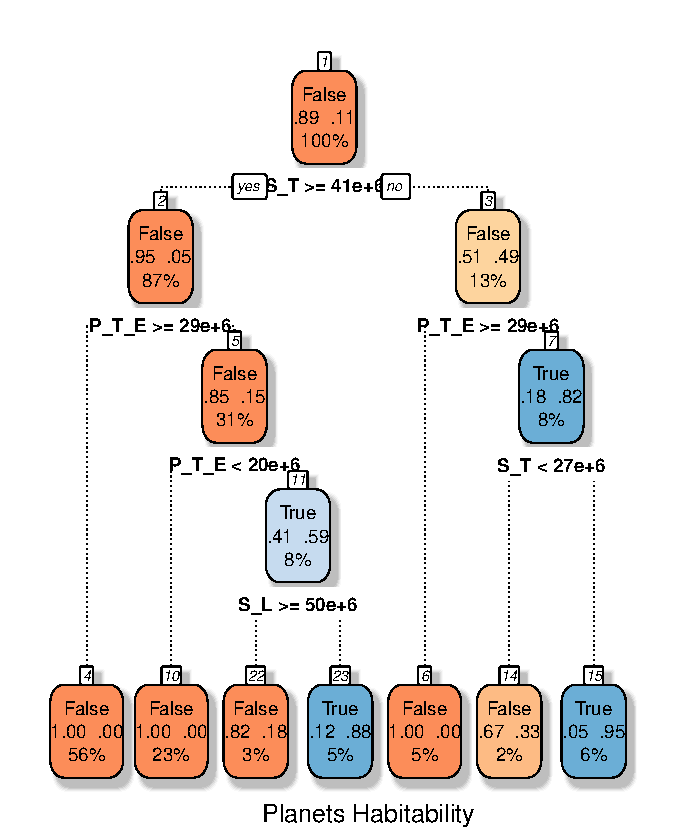
\includegraphics[width=0.8\linewidth]{Pic/DecisionTree.pdf}
\end{center}
\column{0.5\textwidth}
\begin{center}
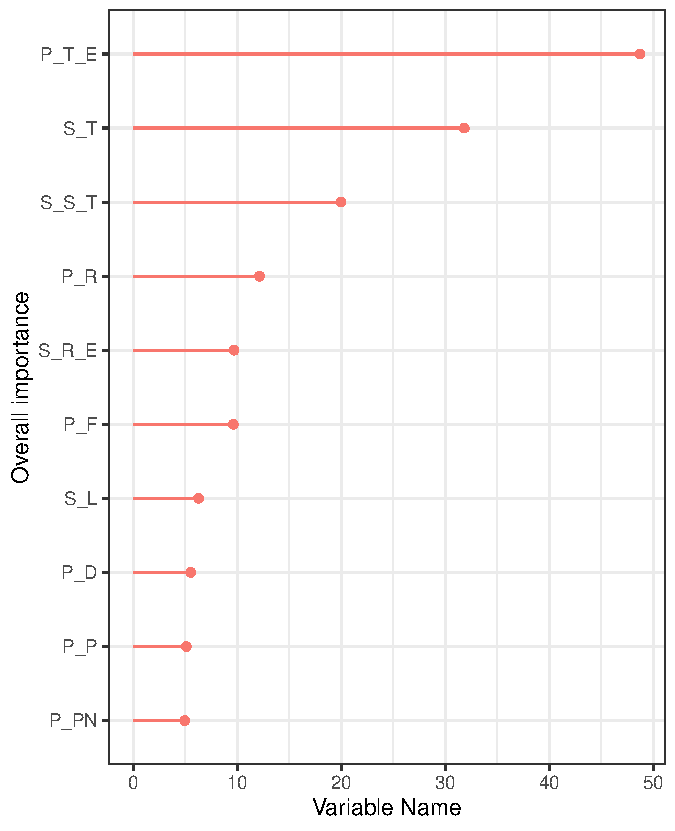
\includegraphics[width=0.5\linewidth]{Pic/Var_imp_dec_tree.pdf}
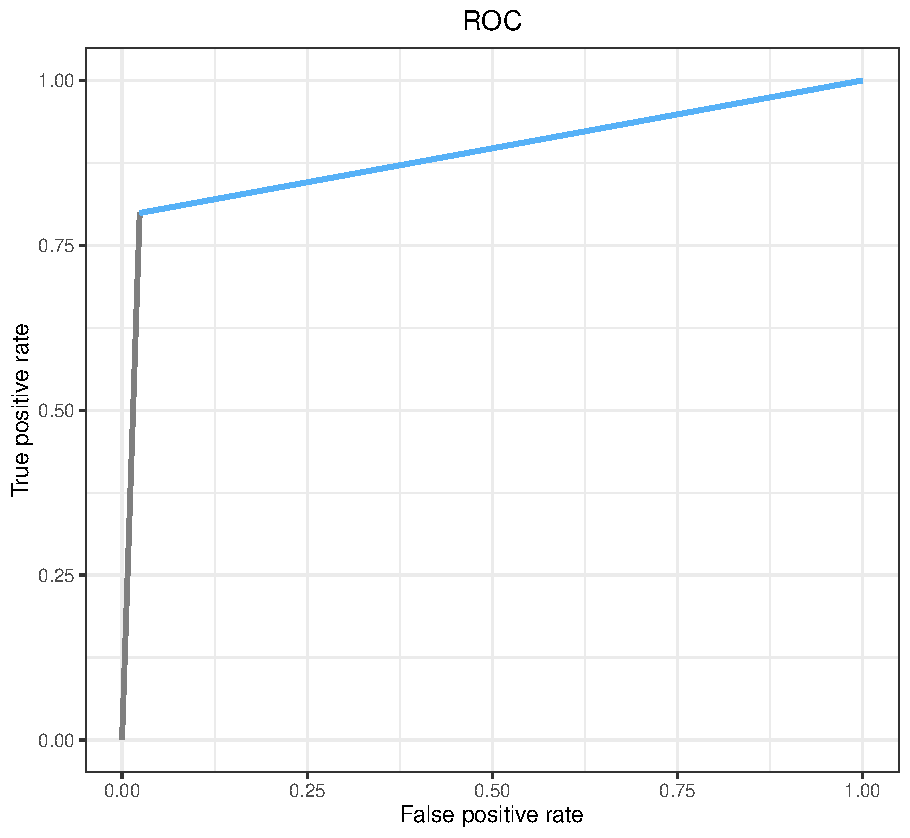
\includegraphics[width=0.5\linewidth]{Pic/Decision_Tree_FINAL_ROC.pdf}\\
$\phi_{DT}=0.790$
\end{center}
\end{columns}
\end{frame}


\subsection{Results - Random Forest}
\begin{frame}
\frametitle{Results - Random Forest}
\begin{columns}
\column{0.5\textwidth}
\begin{center}
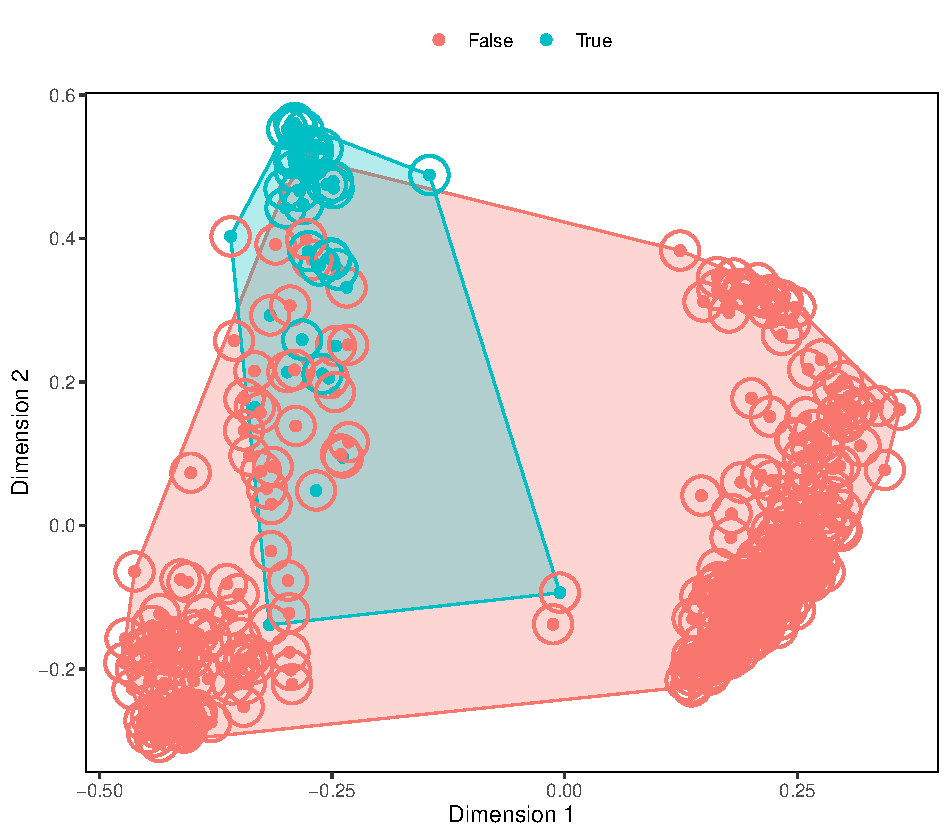
\includegraphics[width=\linewidth]{Pic/Proximity_Random_forest.pdf}
\end{center}
\column{0.5\textwidth}
\begin{center}
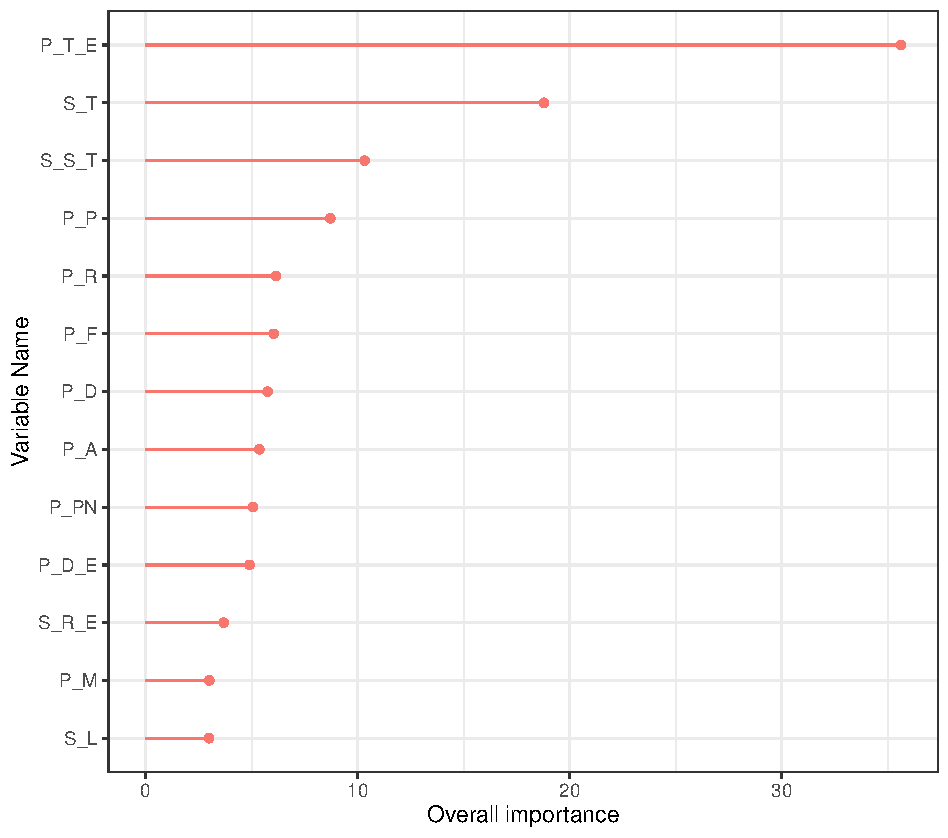
\includegraphics[width=0.6\linewidth]{Pic/Random_forest_importance.pdf}
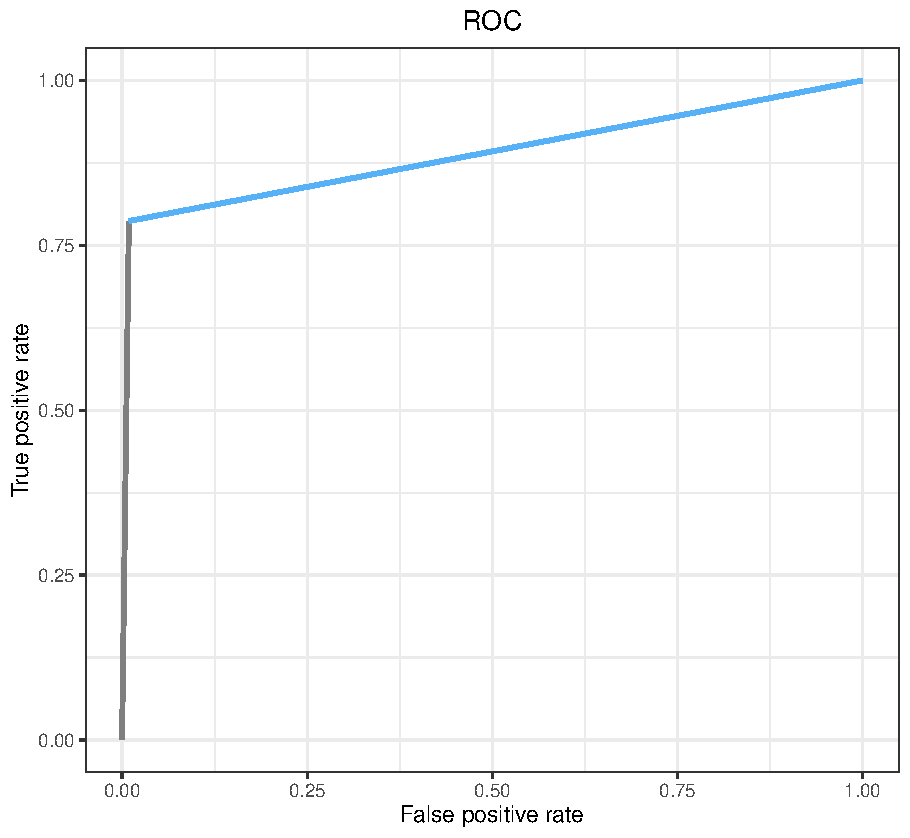
\includegraphics[width=0.6\linewidth]{Pic/Random_Forest_FINAL_ROC.pdf}\\
$\phi_{RF}=0.835$
\end{center}
\end{columns}
\end{frame}

\subsection{Results - SVC}
\begin{frame}
\frametitle{Results - Support Vector Classifier}
\begin{columns}
\column{0.5\textwidth}
\begin{center}
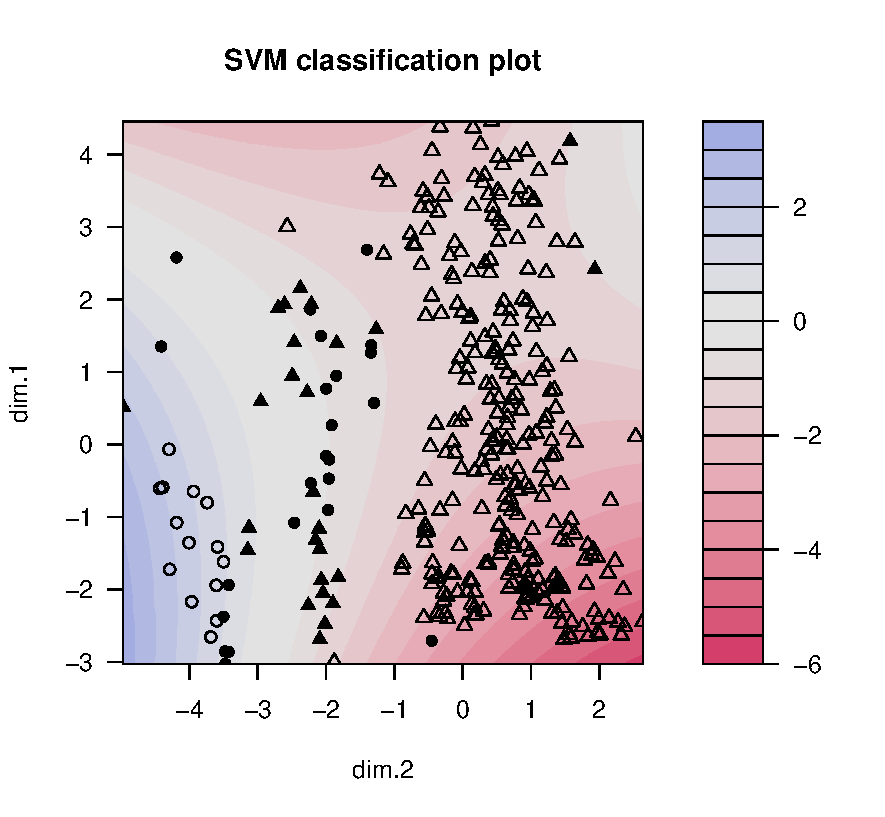
\includegraphics[width=\linewidth]{Pic/PCA+SVM_PLOT.pdf}
\end{center}
\column{0.5\textwidth}
\begin{center}
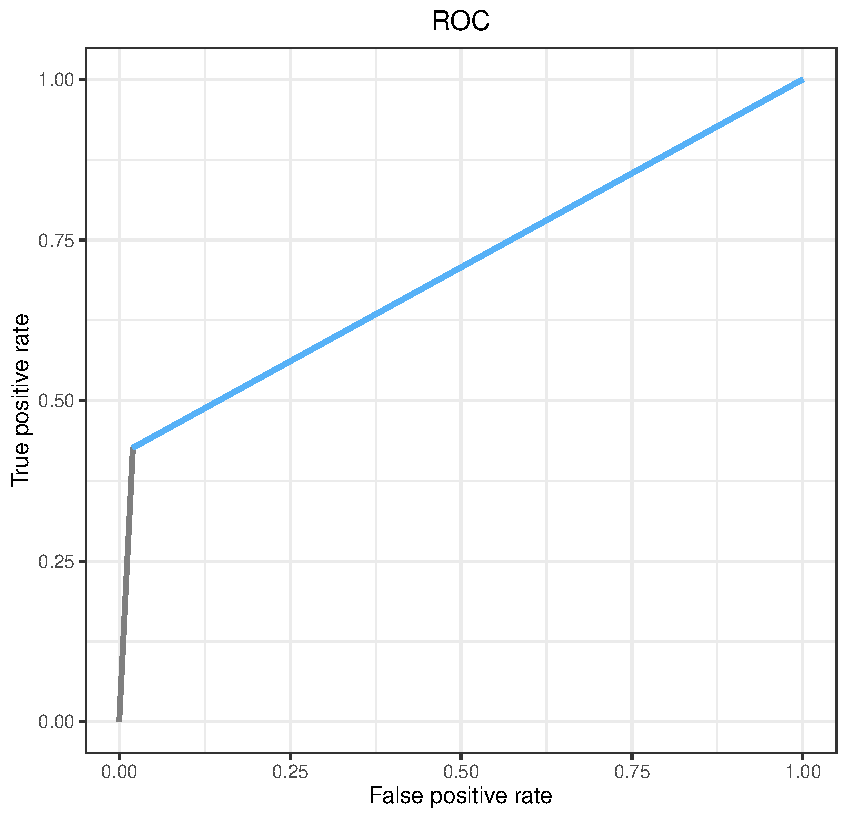
\includegraphics[width=0.5\linewidth]{Pic/SVM_FINAL_ROC.pdf}
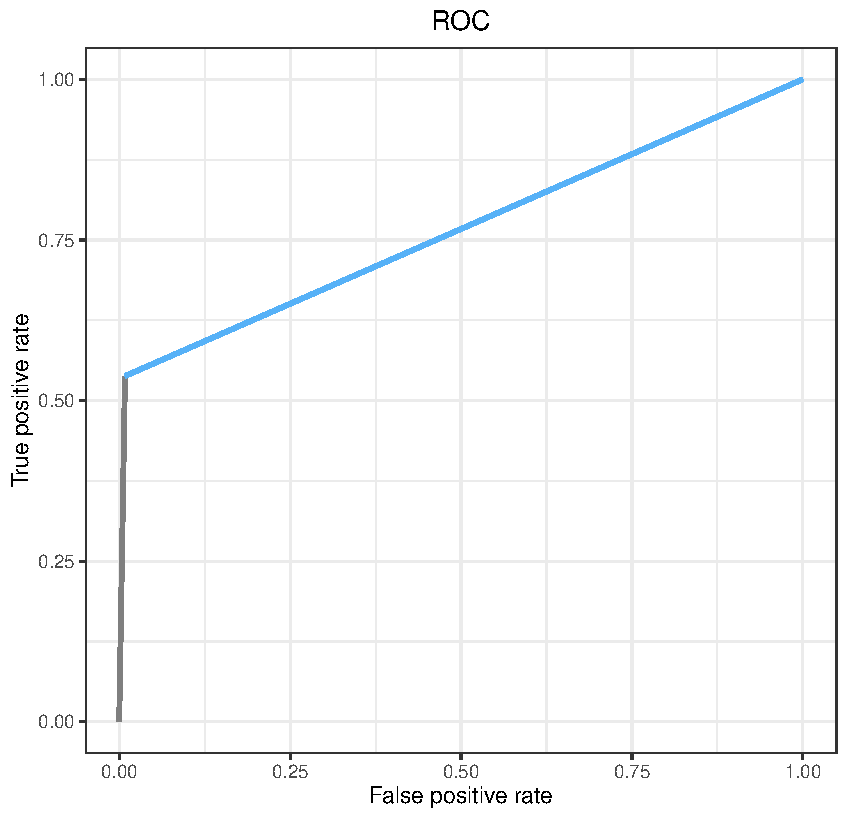
\includegraphics[width=0.5\linewidth]{Pic/SVM_PCA_ROC.pdf}\\
$\phi_{SVC}=0.527$\quad$\phi_{PCA+SVC}=0.667$
\end{center}
\end{columns}
\end{frame}

\subsection{Results - Logistic Classification}
\begin{frame}
\frametitle{Results - Logistic Classification}
\begin{columns}
\column{0.5\textwidth}
\begin{center}
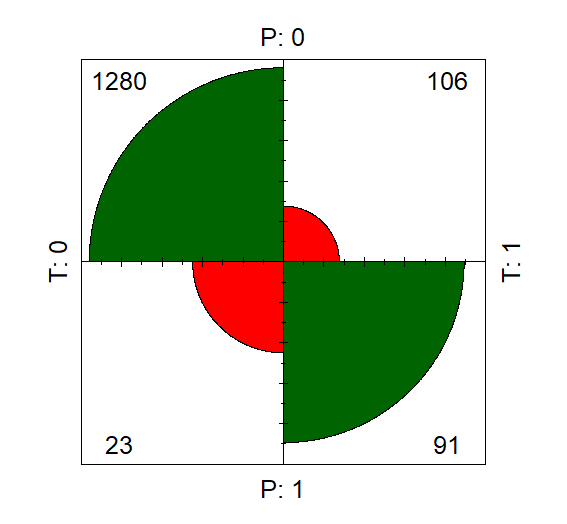
\includegraphics[width=\linewidth]{Pic/LOG_FULL.png}
\end{center}
\column{0.5\textwidth}
\begin{center}
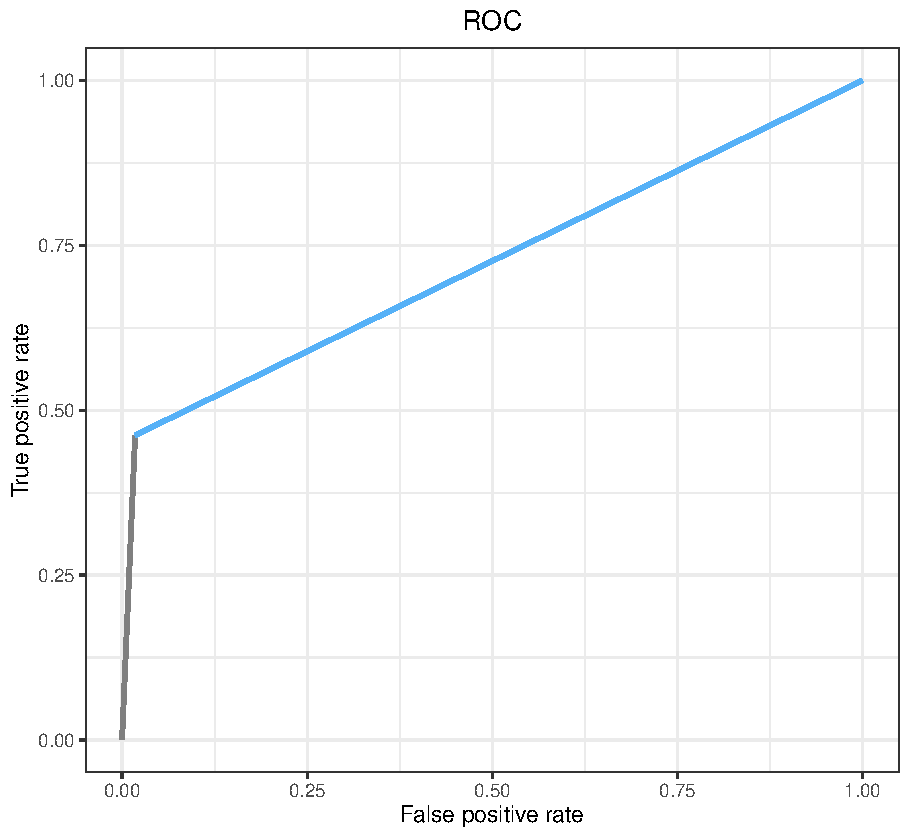
\includegraphics[width=0.85\linewidth]{Pic/LOG_FULL_ROC.pdf}\\
\end{center}
\end{columns}
\begin{center}
$\phi_{log}=0.566$
\end{center}
\end{frame}


\subsection{Results -  LDA and QDA}
\begin{frame}
\frametitle{Results - Linear and quadratic discriminant analysis}
\begin{columns}
\column{0.5\textwidth}
\begin{center}
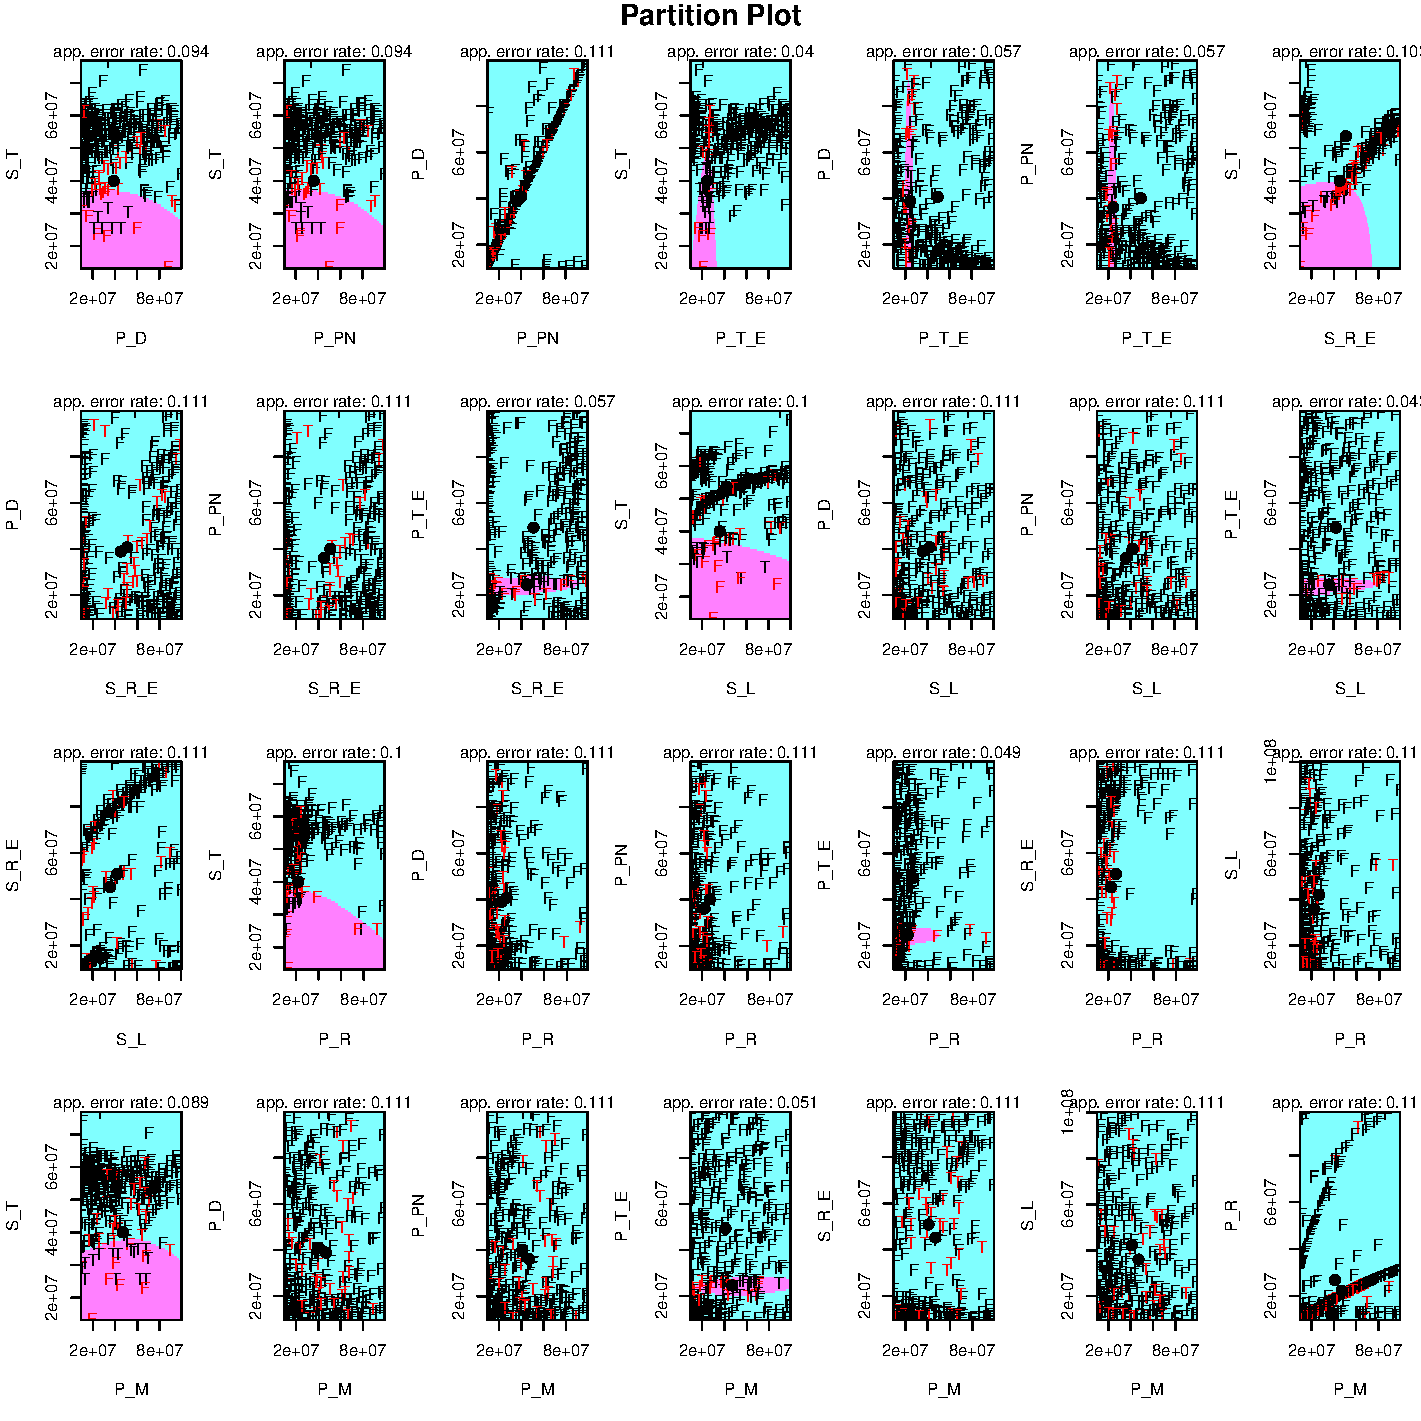
\includegraphics[width=\linewidth]{Pic/QDA_project_FULL.pdf}
\end{center}
\column{0.5\textwidth}
\begin{center}
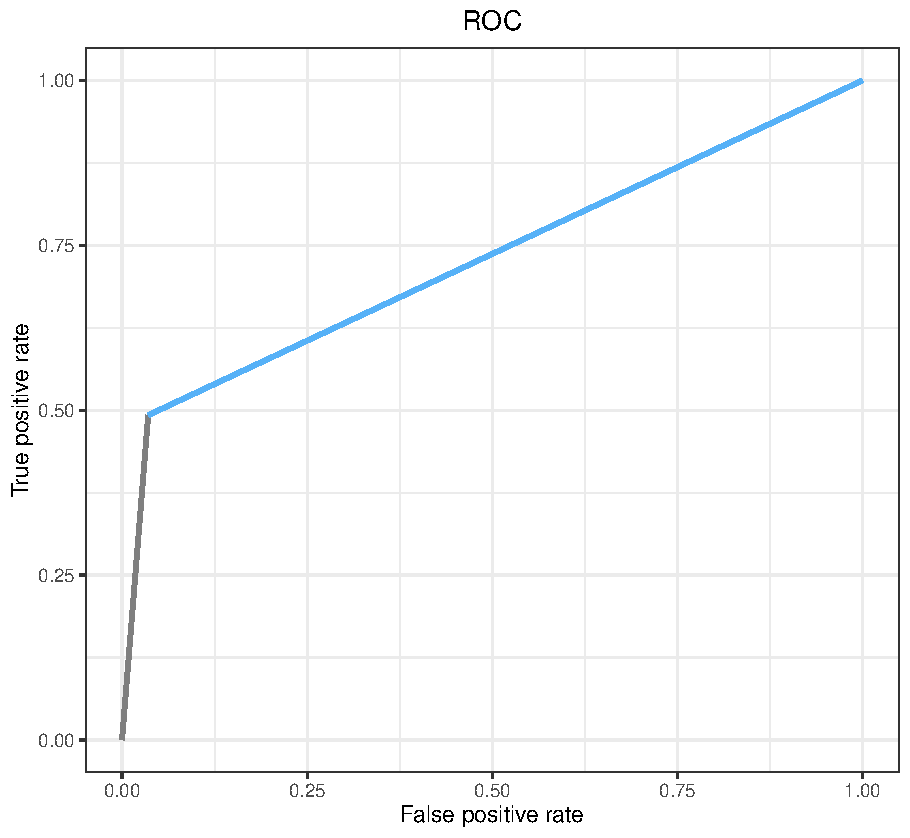
\includegraphics[width=0.5\linewidth]{Pic/LDA_FULL_ROC.pdf}
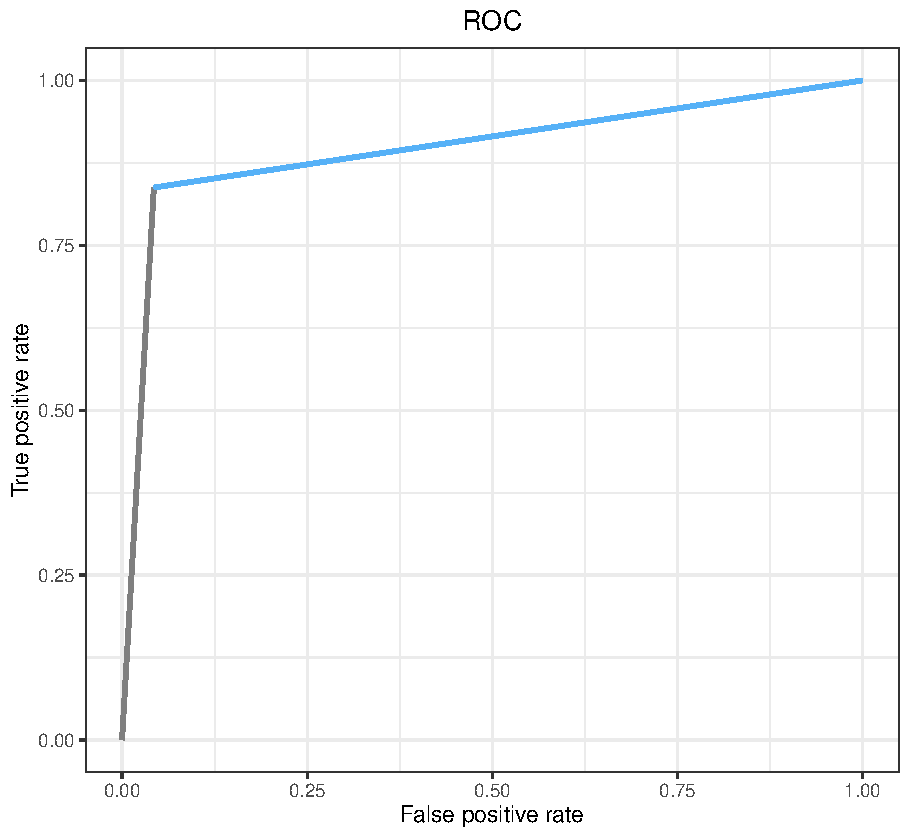
\includegraphics[width=0.5\linewidth]{Pic/QDA_FULL_ROC.pdf}\\
$\phi_{LDA}=0.526$\quad$\phi_{QDA}=0.757$
\end{center}
\end{columns}
\end{frame}


\subsection{Discussion}
\begin{frame}
\frametitle{Discussion}
\begin{table}[]
\begin{center}
\begin{tabular}{c||c|c|c}
{\color[HTML]{CB0000} \textbf{Algortim}} & {\color[HTML]{CB0000} \textbf{Accuracy}} & {\color[HTML]{CB0000} \textbf{NIR}} & {\color[HTML]{CB0000} \textbf{$\phi$}} \\ \hline\hline
Decision tree                            & 0.952                                    & 0.867                               & 0.790                                  \\ \hline
Random forest                            & 0.964                                    & 0.869                               & 0.835                                  \\ \hline
SVM                                      & 0.907                                    & 0.869                               & 0.527                                  \\ \hline
PCA+SVM                                  & 0.932                                    & 0.869                               & 0.667                                  \\ \hline
Logistic                                 & 0.914                                    & 0.869                               & 0.566                                  \\ \hline
LDA                                      & 0.902                                    & 0.898                               & 0.526                                  \\ \hline
QDA                                      & 0.941                                    & 0.869                               & 0.757 
                             
\end{tabular}
\end{center}
\end{table}
\begin{itemize}
\item The random forest algorithm provides the best forecast, followed by the decision tree and the the QDA. 
\item This behaviour can be explained by considering that in the features space,as showed in the previous plots, the two sets largely overlaps
\item A similar performance ranking was found by Sasha et al. (2018) \cite{saha2018machine}

\end{itemize}
\end{frame}

\begin{frame}
\begin{center}
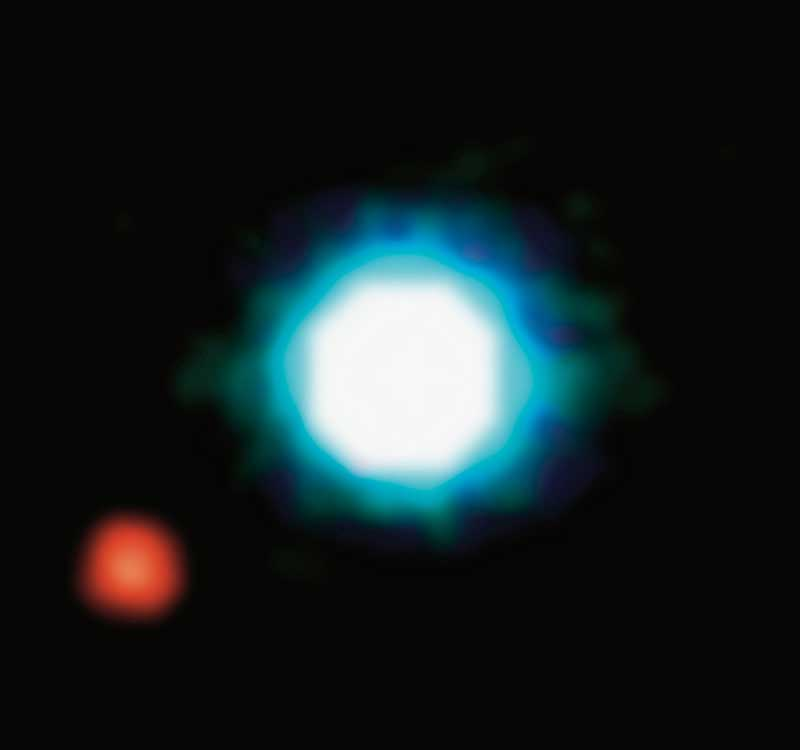
\includegraphics[width=0.5\linewidth]{Pic/Exoplanet_picture.jpg}
\end{center}
\begin{center}
The 2M1207b exoplanet (red spot) and its host star 2M120 (a brown dwarf) as observed, after three near-infrared exposures (H, K and L wavebands), by the VLT Yepun telescope at the ESO Paranal Observatory. Image taken from \cite{exoplanet_pic}
\end{center}
\end{frame}

\begin{frame}
\begin{center}
\textit{Per aspera ad astra}
\end{center}
\end{frame}



\begin{frame}[t,allowframebreaks]
\frametitle{References}
\printbibliography
\end{frame}

\section{Supporting slides}
\begin{frame}
\begin{center}
SUPPORTING SLIDES
\end{center}
\end{frame}

\begin{frame}
\frametitle{Proximity plot - Explanation}
\begin{center}
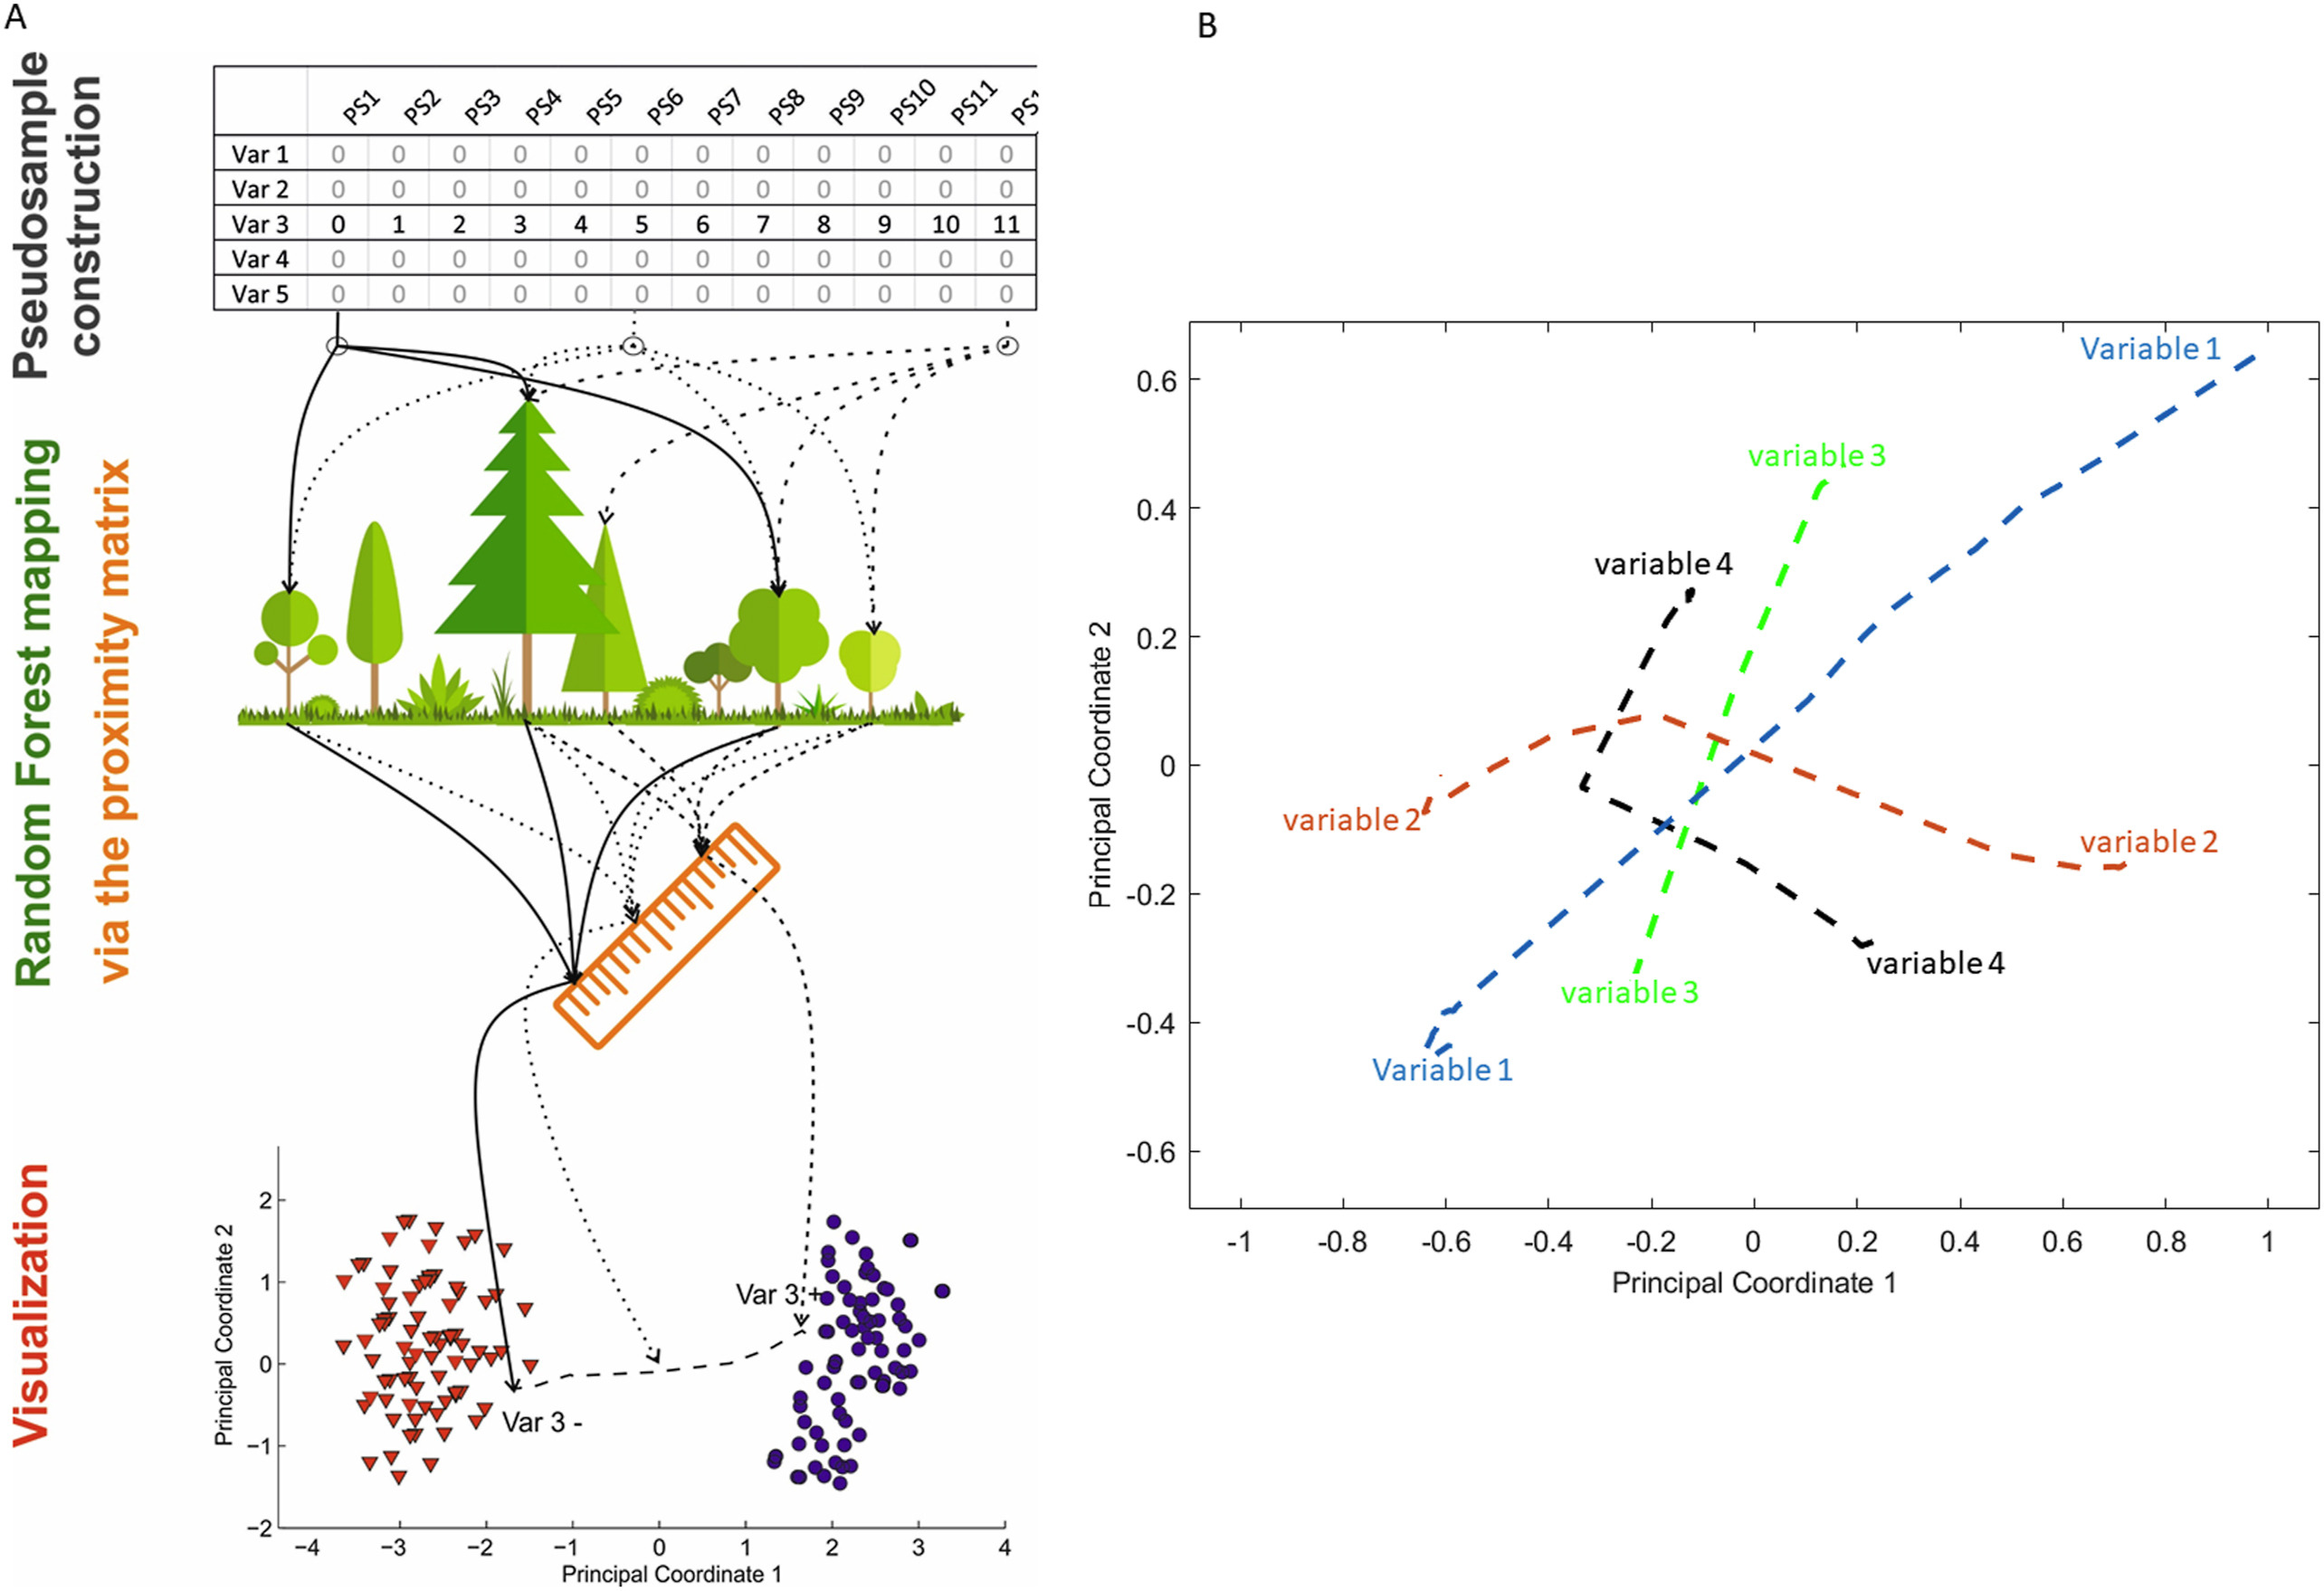
\includegraphics[width=0.8\linewidth]{Pic/Prox_explanation.jpg}\\
Image taken from \cite{blanchet2020constructing}
\end{center}
\end{frame}

\begin{frame}
\begin{center}
\frametitle{Proximity plot - Explanation}
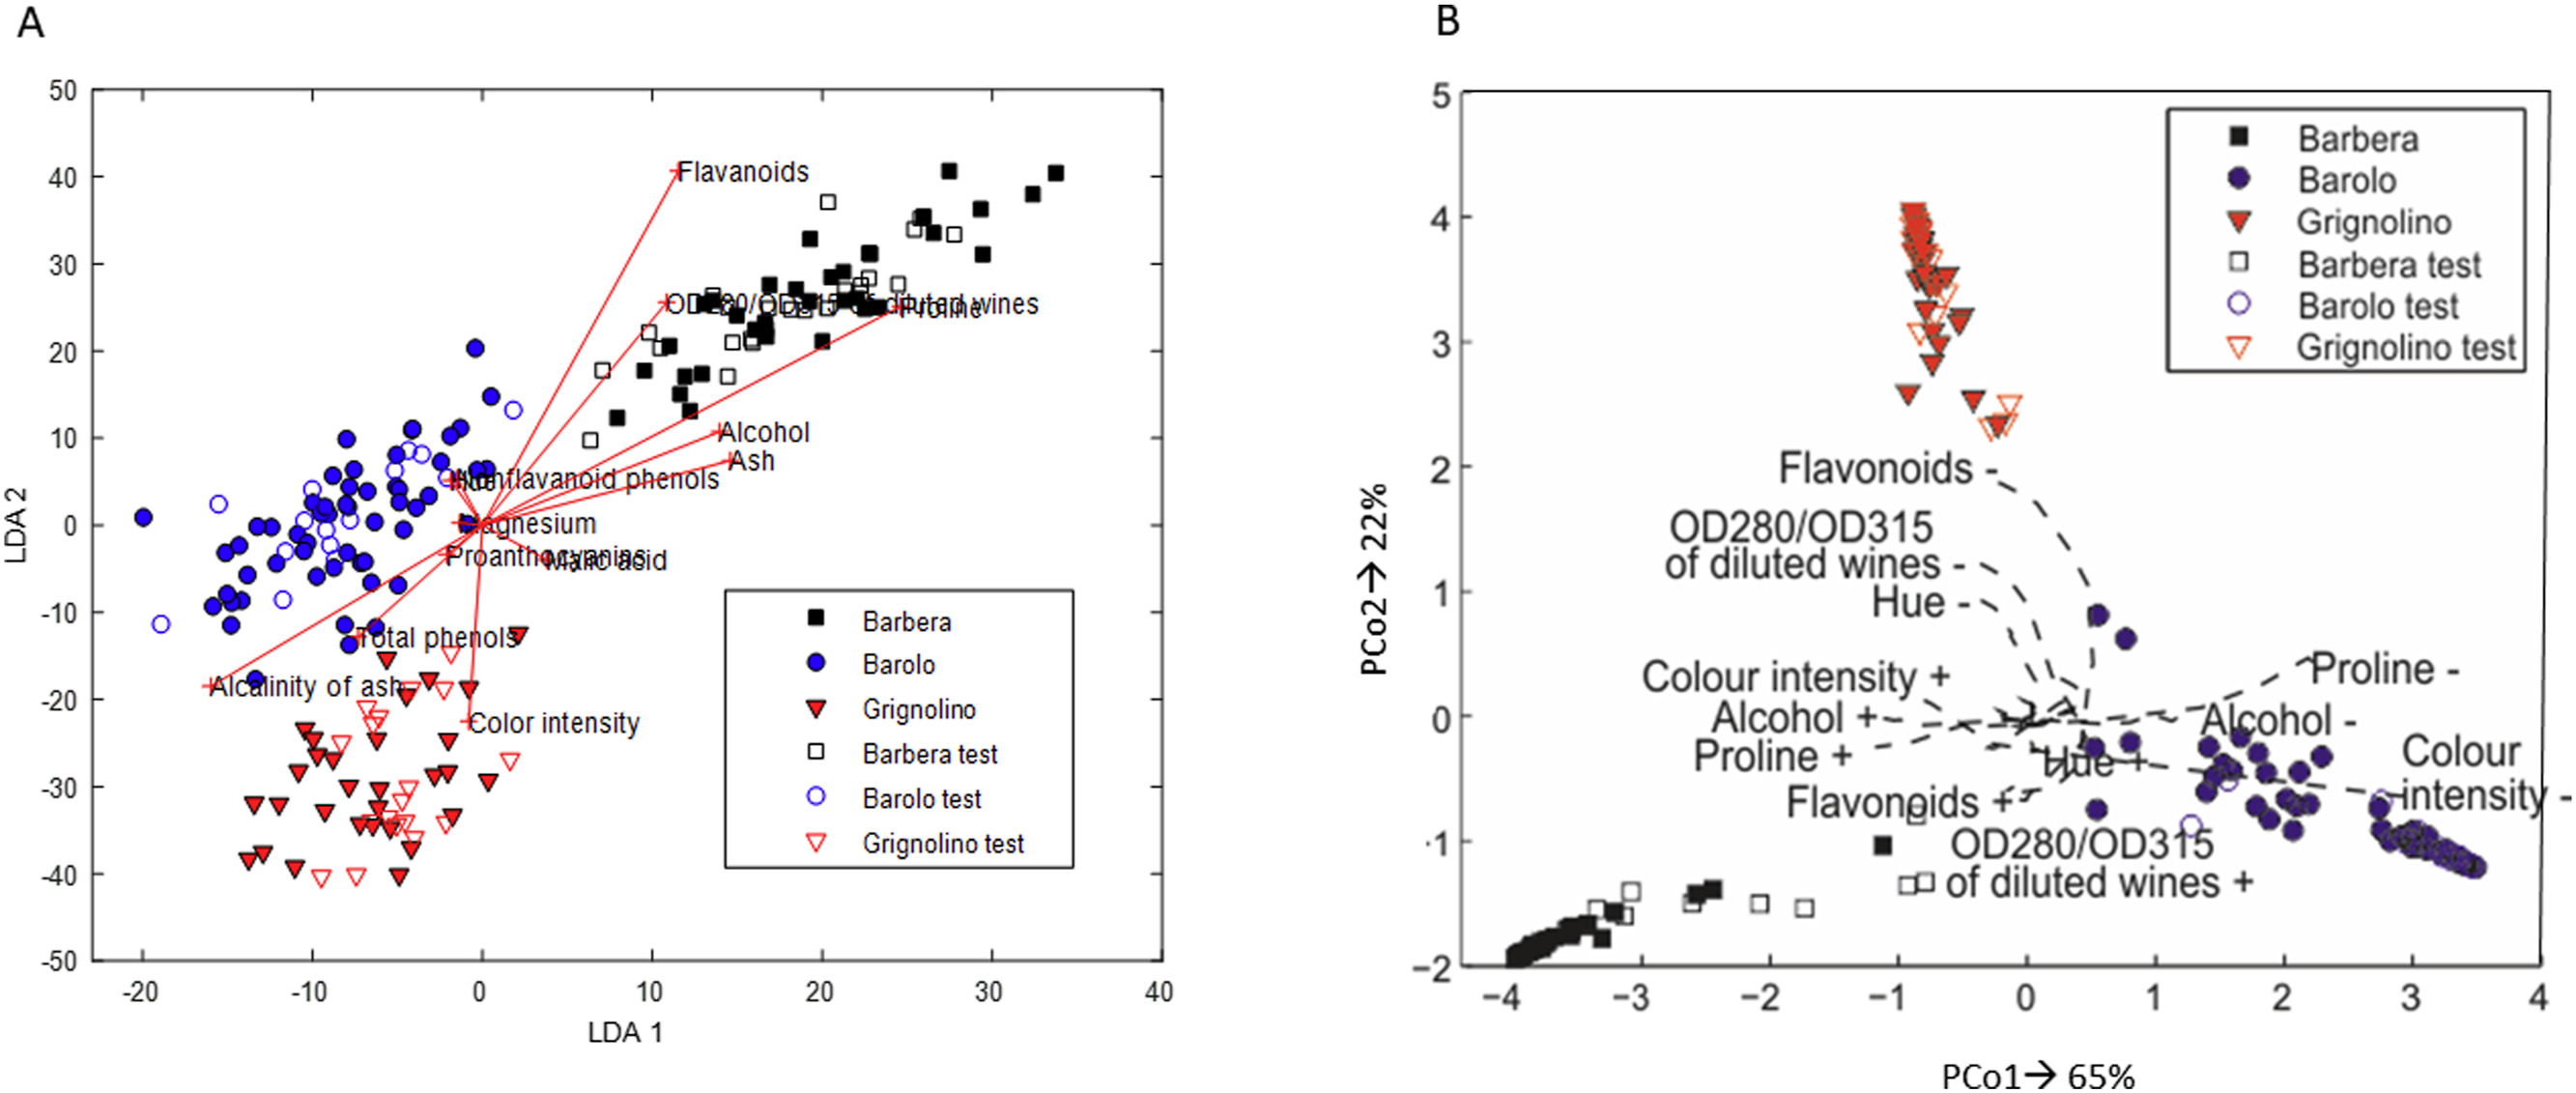
\includegraphics[width=0.8\linewidth]{Pic/Prox_explanation_3.jpg}\\
Image taken from \cite{blanchet2020constructing}
\end{center}
\end{frame}

\begin{frame}
\begin{center}
\frametitle{Proximity plot - Explanation}
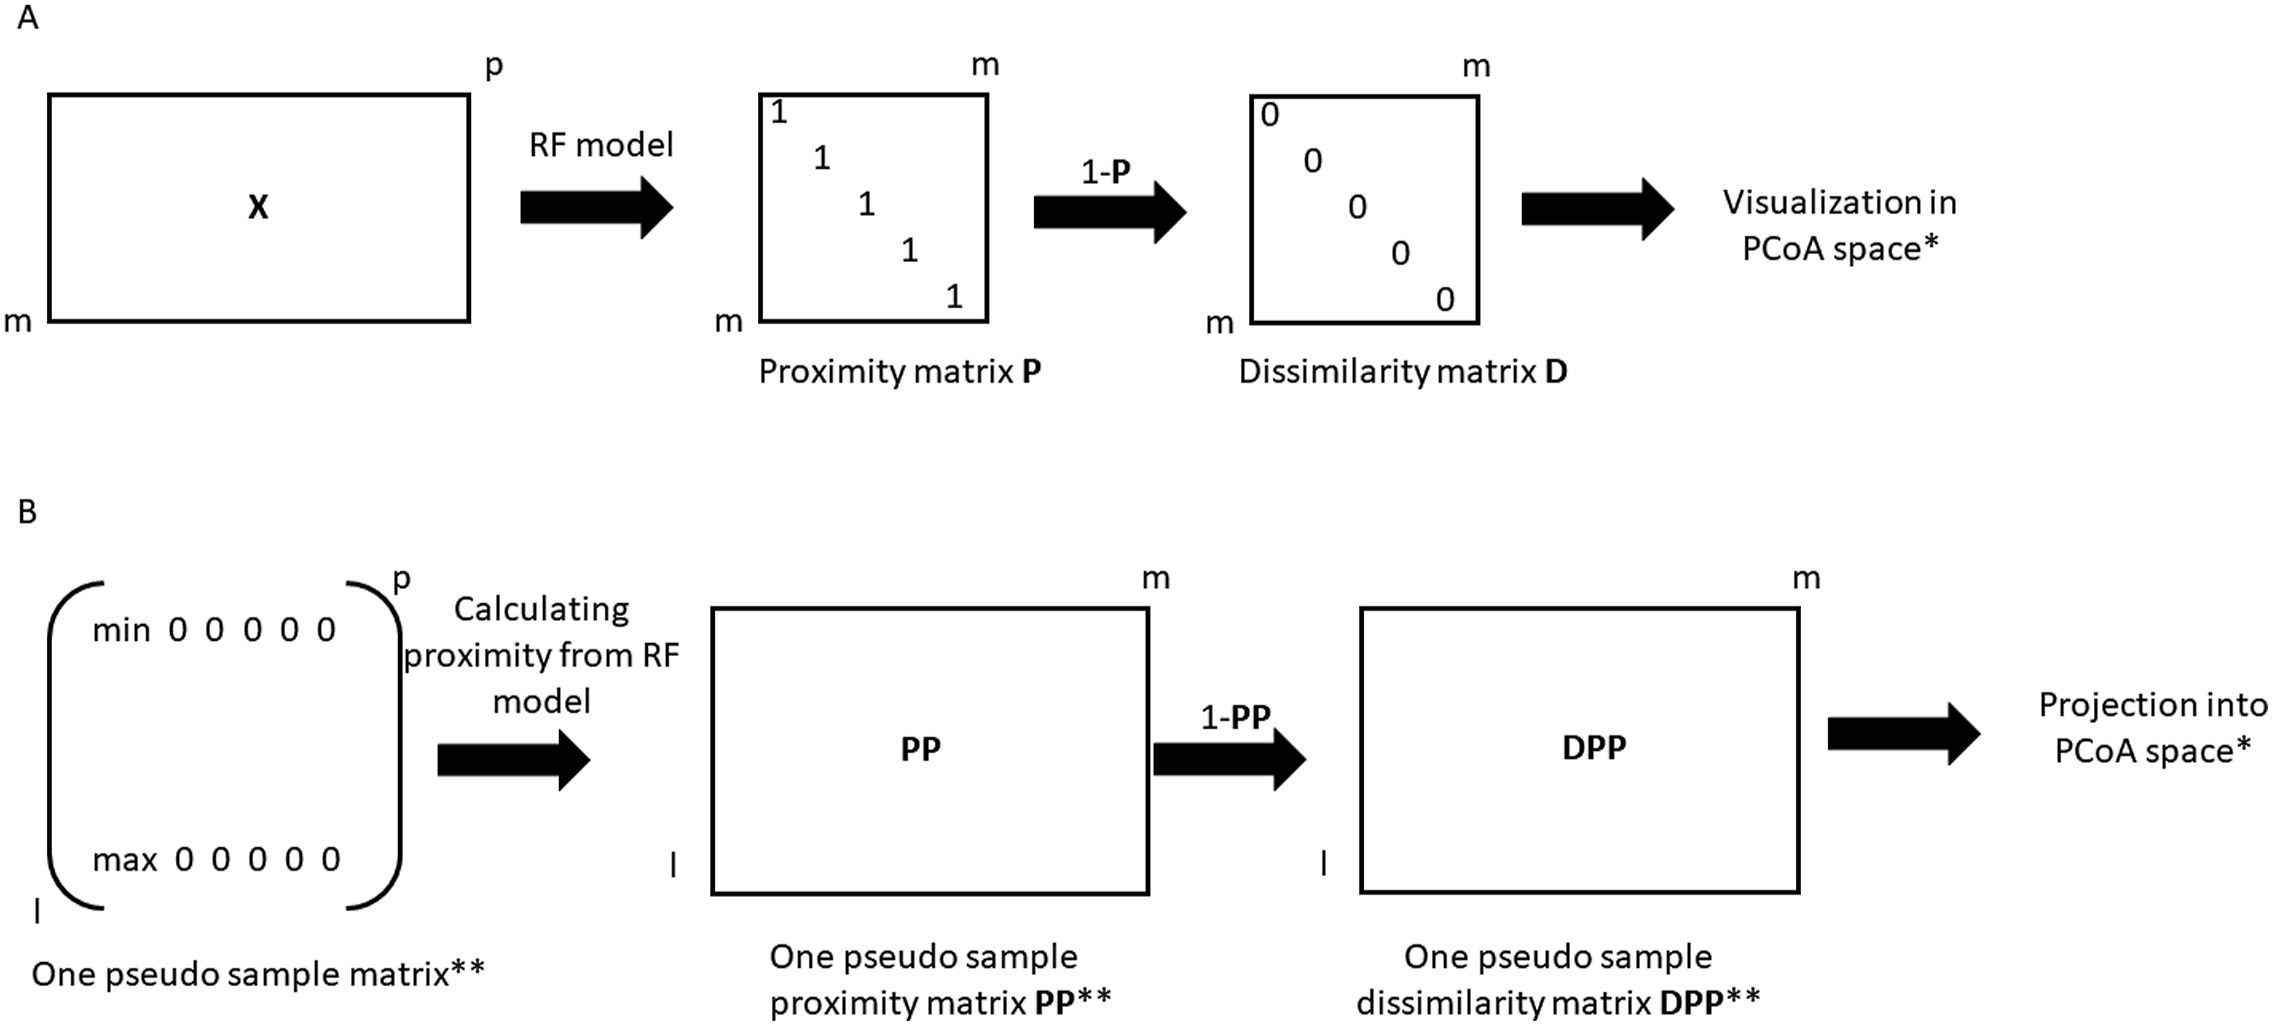
\includegraphics[width=0.8\linewidth]{Pic/Prox_explanation_2.jpg}\\
Image taken from \cite{blanchet2020constructing}
\end{center}
\end{frame}

\begin{frame}
\begin{center}
\frametitle{$\phi$ coefficent}
\begin{table}[]
\begin{tabular}{c|c|c}
\multicolumn{1}{l|}{\textbf{}} & \textbf{Actual - N} & \textbf{Actual - P} \\ \hline
\textbf{Predicted - N}         & \#TP                & \#FN                \\ \hline
\textbf{Predicted - P}         & \#FP                & \#TP               
\end{tabular}
\end{table}
\begin{equation*}
\phi=\dfrac{TP\times TN - FP\times FN}{\sqrt{\left(TP+FP\right)\left(TP+FN\right)\left(TN+FP\right)\left(TN+FN\right)}}
\end{equation*}
\end{center}
\end{frame}

\end{document}